\documentclass[a4paper, 12pt]{article}

\usepackage[croatian]{babel}
\usepackage[utf8]{inputenc}
\usepackage[unicode]{hyperref}
\usepackage{appendix}
\usepackage[section, notlof]{tocbibind}
\usepackage{graphicx}
\usepackage{csquotes}
\usepackage[super,square]{natbib}
\usepackage{lastpage}
\usepackage{setspace}
\usepackage{longtable}
\usepackage{makecell}
\usepackage{multirow}
\usepackage{geometry}
\geometry{
	top=1in,
	inner=1in,
	outer=1in,
	bottom=1in,
	headheight=0.3in,
	headsep=0.4in,
}
\usepackage{fancyhdr}

\setlofname{Indeks}
\renewcommand{\contentsname}{Sadržaj}
\renewcommand\refname{Literatura}
\pagestyle{fancy}

\rhead{}
\lhead{}
%\lfoot{}
\cfoot{\thepage{} od \pageref{LastPage}}
\rfoot{\textless Datum\textgreater}

\renewcommand{\footrulewidth}{1pt}
\renewcommand{\headrulewidth}{1pt}
\begin{document}
\thispagestyle{fancy}
	\begin{titlepage}
	 \thispagestyle{empty}
	 \setstretch{2}
	 \vspace*{5\baselineskip}
	 \centerline{\huge \textless Naziv projekta\textgreater}
	 \vspace*{3\baselineskip}
	 \centerline{\Large \textbf{Studentski tim:} Dubravko Lukačević }
	 \centerline{\hspace{4.7cm} \Large Dominik Marjanović }
	 \centerline{\hspace*{4.5cm} \Large Tomislav Markovac }
	 \centerline{\hspace{3.1cm} \Large Josip Trbuščić}
	 \vspace*{4\baselineskip}
	 \centerline{\Large \textbf{Mentor:} izv. prof. dr. sc. Miljenko Mikuc}
\end{titlepage}



	\addtocounter{page}{1}

	\newpage
	\tableofcontents
	
	\newpage
	\section{Uvod}
	\hspace{0.5cm}
Virtualna privatna mreža (engl. VPN, virtual private network) je tehnologija koja omogućava sigurno povezivanje privatnih mreža preko javne mrežne infrastrukture. VPN je razvijen kako bi se geografski udaljenim korisnicima omogućio siguran pristup privatnoj mreži.\cite{cis} Do potrebe za takvom tehnologijom je došlo devedesetih godina te se ona u početku razvijala samo za velike organizacije koje su zahtijevale siguran prijenos osjetljivih podataka putem interneta. Kroz godine komercijalizacija interneta omogućila je većini država pristup najvećoj mreži što je drastično povećalo broj potencijalnih žrtava tadašnjih hakera. Nakon brojnih provala u sustave velikih tvrtki svakodnevni korisnici postali su svjesni loše sigurnosti interneta zbog čega raste potražnja tehnologija koje poboljšavaju mrežnu sigurnost.
 \bigbreak
	
Zaštita podataka osigurava se šifriranjem i dodavanjem posebnih zaglavlja na postojeći paket kako bi se osigurala njegova  autentičnost, integritet i povjerljivost, koji su neki od osnovnih sigurnosnih zahtjeva. Šifriranje se odnosi na  postupak pretvaranja izvornog teksta u šifrirani tekst pri čemu se koriste ključevi i prikladni algoritmi (npr. AES, RSA). Obrnuti proces, dešifriranje, provodi se kako bi samo korisnik koji posjeduje odgovarajući ključ mogao čitati izvoran tekst. U kontekstu mrežne sigurnosti šifriranje koristimo za zaštitu zaglavlja i podataka koji se nalaze unutar paketa.\cite{fundamentals} 
\bigbreak

Jedan od najpoznatijih i najsigurnijih skupova protokola koji se koristi u VPN tehnologijama je sigurni IP (engl. Internet Protocol Security, IPsec). IPsec uključuje protokole mrežnog sloja kako bi se omogućila sigurna razmjena podataka između parova mreža (engl. network-to-network), računala (engl. host-to-host) ili računala i mreža (netowrk-to-host). Neki od korištenih protokola su AH (engl. Authentication Header) kojim se postiže autentičnost paketa i ESP (engl. Encapsulating Security Payload) čija je zadaća da osigura povjerljivost podataka i informacija. Uz IPsec često korišteni skupovi protokola su: OpenVPN, PPTP, SoftEther i WireGuard. 
\bigbreak
 
U današnje vrijeme moguće je birati između mnogo pružatelja VPN usluga od kojih su neki besplatni dok su ostali dostupni kroz mjesečne ili godišnje pretplate. Besplatne se VPN usluge možda čine kao dobro rješenje za siguran prijenos podataka, ali pružatelje takvih usluga ništa ne sprječava od prodaje naših podataka ili korištenja istih u vlastitu korist. Još jedna opcija je postavljanje vlastitog VPN poslužitelja što može izgledati kao dugotrajan i naporan posao, ali ovakvo nam rješenje omogućava da sami odlučimo kako želimo zaštititi prijenos vlastitih podataka. U ostatku rada nalazi se pregled, usporedba i upute za instalaciju poznatijih VPN tehnologija na različitim platformama.



	\newpage
	\section{Windows}
	\subsection{Windows 10 VPN}
	

	
	\newpage
	\subsection{SoftEther VPN}
	\bigbreak
\paragraph*{Što je SoftEther VPN?}
\hfill \smallbreak
\begin{wrapfigure}{r}{0.5\textwidth} 
     \centering
     
\includegraphics[width=0.5\textwidth]{SoftEther/SoftEtherLogo}
	\caption{Službeni logo SoftEther VPN-a}
\end{wrapfigure}

SoftEther VPN\cite{softether} besplatan je višeplatformski program otvorenog koda koji podržava korištenje različitih VPN protokola. Program je nastao 2013. godine kao akademski projekt na sveučilištu u Tsukubi i podržan je na različitim operacijskim sustavima kao što su Linux, FreeBSD, Mac, Solaris i Windows za koji je u ovom poglavlju prikazan postupak postavljanja i uporabe.
\smallbreak
Program SoftEther otvorenog je koda pa ga može bilo tko koristiti za vlastite ili komercijalne svrhe.\smallbreak
SoftEther VPN koristi HTTPS preko SSL (Secure Sockets Layer)\cite{ssl}
protokola kako bi omogućio siguran prijenos kriptiranih podataka preko Interneta. Uz njega su podržani unutar programa i ostali poznatiji protokoli kao što su OpenVpn, IPsec, L2TP, ...\\
Unutar programa sve postavke detaljno su objašnjene i mogu se podesiti korištenjem grafičkog sučelja što ovaj program čini jednostavnim za uporabu.

\FloatBarrier

\bigbreak
\paragraph*{Instalacija SoftEther servera}

\hfill \smallbreak
Za početak potrebno je preuzeti instalaciju VPN servera sa službene stranice SoftEthera:\\ \url{https://www.softether.org}
\begin{figure}[h!]
	\centering
     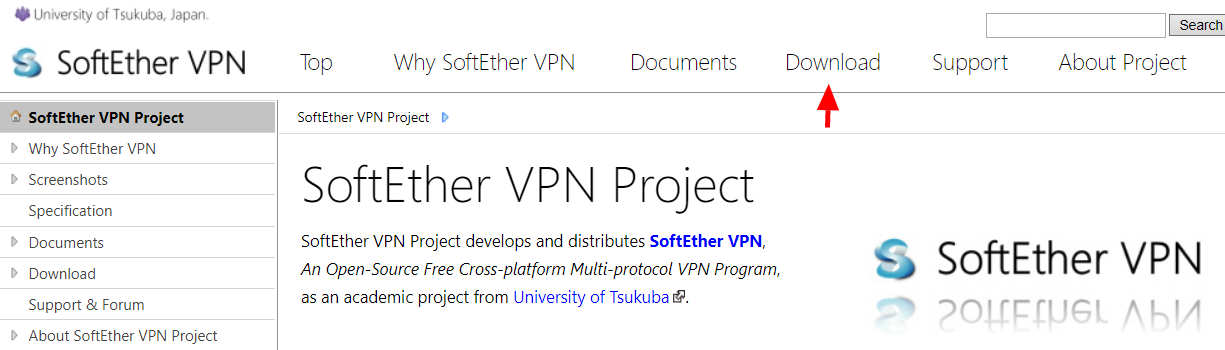
\includegraphics[width=0.6\textwidth]{SoftEther/korak1}
\end{figure}
\FloatBarrier
Odabirom ``Download'' iz izborne trake prikazuje se stranica s ponuđenim poveznicama za preuzimanje.
\begin{figure}[h!]
     \centering
     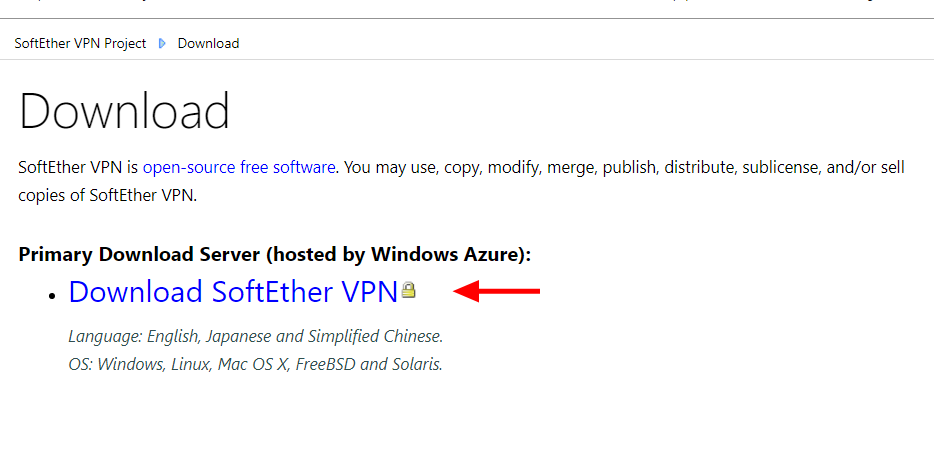
\includegraphics[width=0.6\textwidth]{SoftEther/korak2}
\end{figure}
\FloatBarrier
Sljedeći isječak prikazuje stranicu koja se otvori odabirom prve poveznice. Na stranici se nalaze izborni okviri u kojima je potrebno odabrati željeni program. Za preuzimanje VPN servera potrebno je odabrati postavke prikazane na sljedećem isječku te odabrati prvu poveznicu za početak preuzimanja.
\begin{figure}[h!]
     \centering
     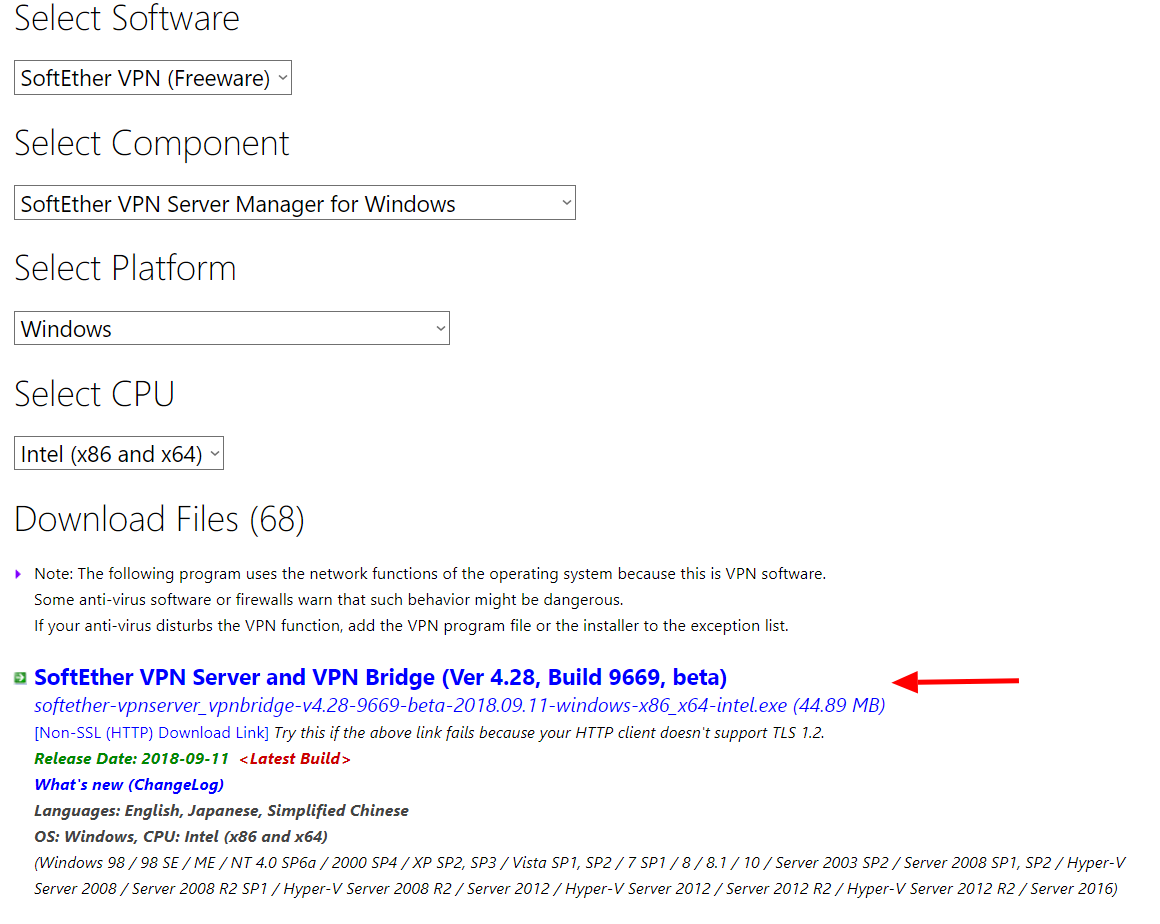
\includegraphics[width=0.6\textwidth]{SoftEther/korak6}
\end{figure}
\FloatBarrier
Nakon preuzimanja i pokretanja instalacije otvara se sljedeći prozor u kojemu se predlaže odabir prvog ponuđenog jer nudi potpunu instalaciju.
\begin{figure}[h!]
     \centering
     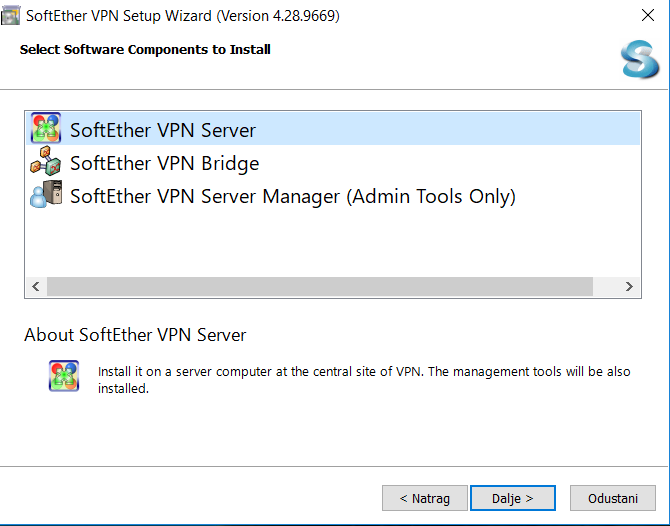
\includegraphics[width=0.6\textwidth]{SoftEther/korak7}
\end{figure}
\FloatBarrier
Nakon uspješne instalacije prikazuje se sljedeći okvir u kojem još nema niti jednog servera. Dodavanje servera započinje se odabirom ``New Setting''.
\begin{figure}[h!]
     \centering
     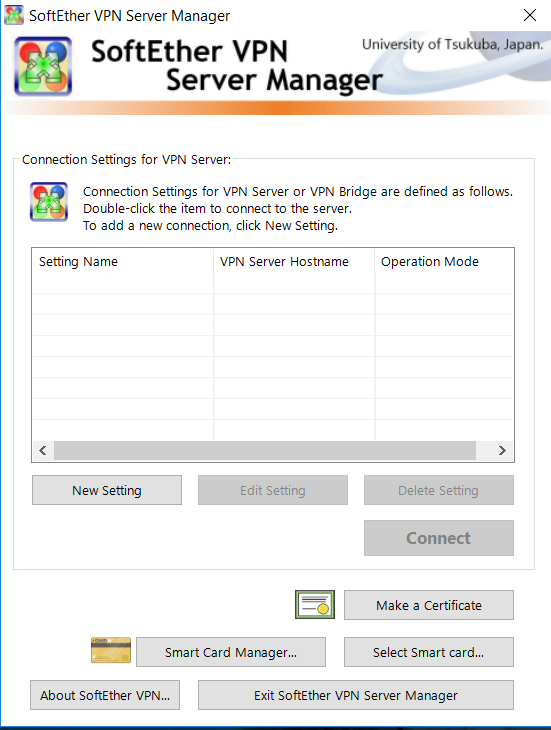
\includegraphics[width=0.6\textwidth]{SoftEther/korak8}
\end{figure}
\FloatBarrier
Stvaranje servera započinje se upisom željenog naziva u polje ``setting name'' i upisom vlastite IP adrese preko koje je trenutno računalo spojeno na Internet. Upute za pronalazak IP adrese mogu se pronaći na kraju ovog poglavlja. Preporuka je dodati lozinku za pristup serveru radi dodatne sigurnosti u polje ``password''.
\begin{figure}[h!]
     \centering
     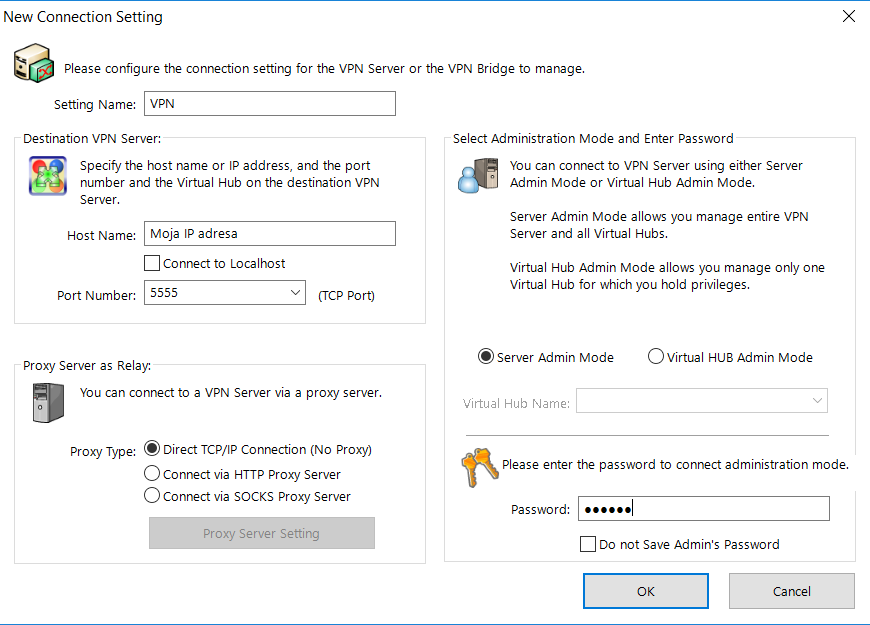
\includegraphics[width=0.6\textwidth]{SoftEther/korak9}
\end{figure}
\FloatBarrier
U tablici sada vidimo da je dodan novi server kojeg je potrebno konfigurirati odabirom ``Connect'' opcije.
\begin{figure}[h!]
     \centering
     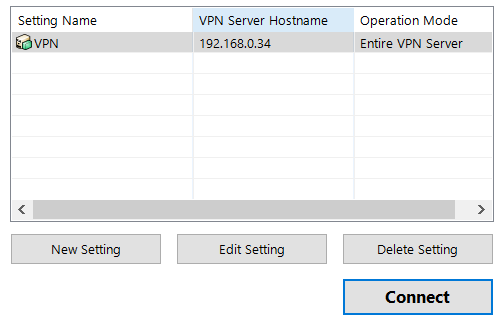
\includegraphics[width=0.6\textwidth]{SoftEther/korak10}
\end{figure}
\FloatBarrier
Kako bi se druga računala uspjela povezati s napravljenim serverom, potrebno je dodati virtualno čvorište odabirom opcije ``Create a Virtual Hub''.
\begin{figure}[h!]
     \centering
     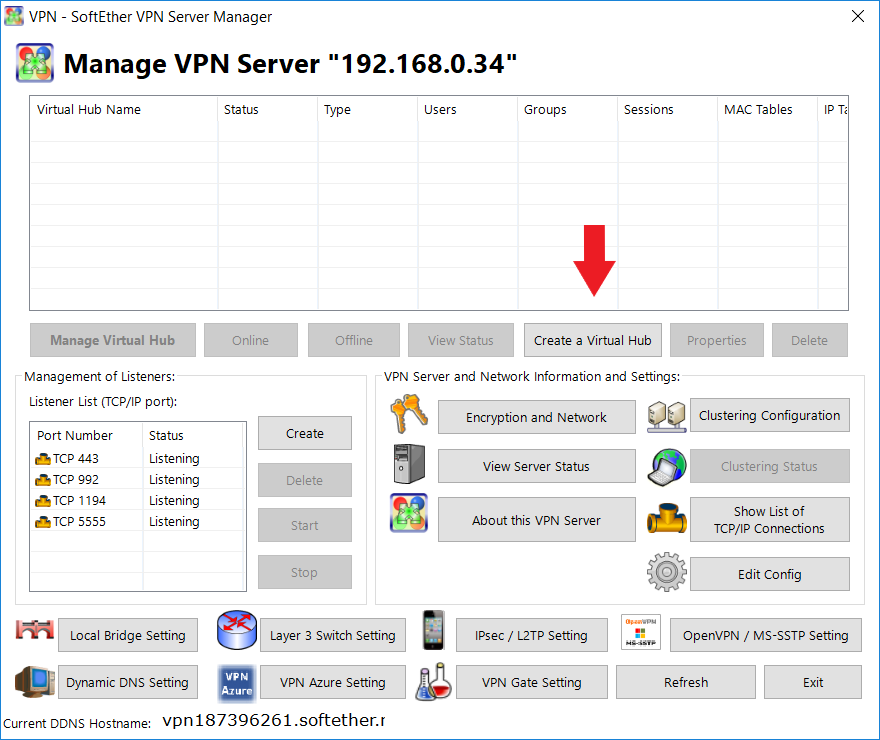
\includegraphics[width=0.6\textwidth]{SoftEther/korak11}
\end{figure}
\FloatBarrier
Virtualnom čvorištu postavljamo proizvoljno ime te dodajemo lozinku radi dodatne sigurnosti.
\begin{figure}[h!]
     \centering
     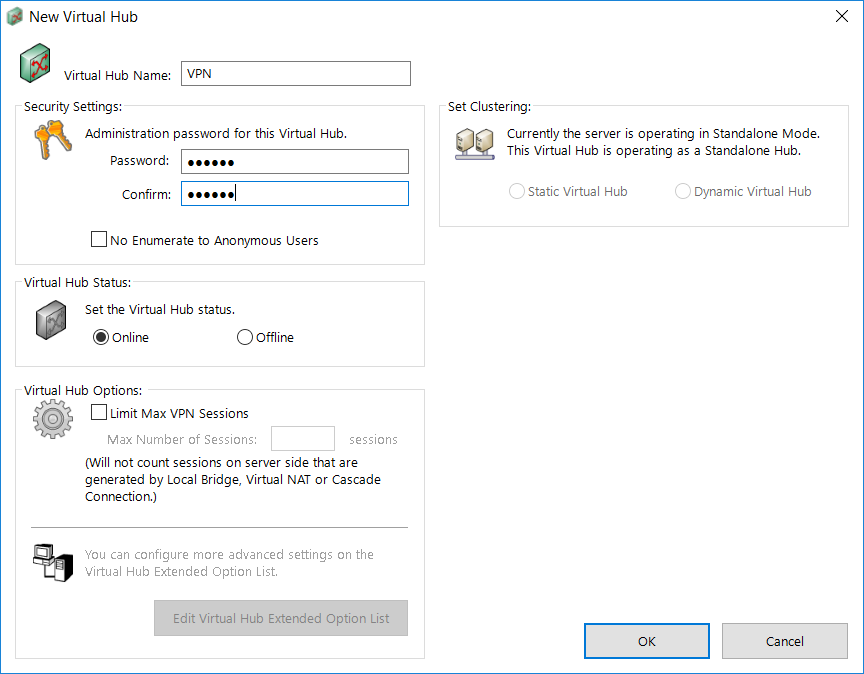
\includegraphics[width=0.6\textwidth]{SoftEther/korak12}
\end{figure}
\FloatBarrier
Sada se može vidjeti novo dodano čvorište u tablici.
\begin{figure}[h!]
     \centering
     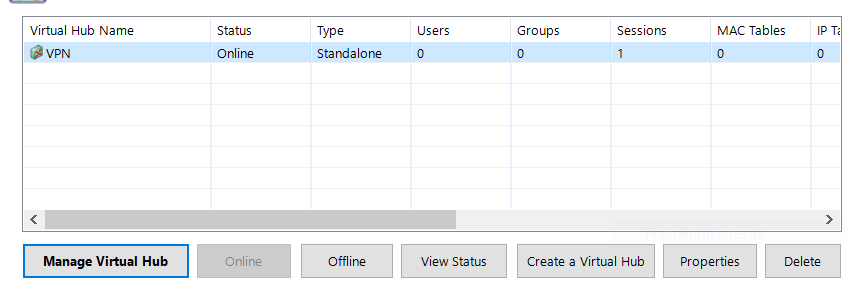
\includegraphics[width=0.6\textwidth]{SoftEther/korak13}
\end{figure}
\FloatBarrier
Sljedeći je korak odrediti tko se sve može povezati na naš server, a to se radi odabirom gumba ``Manage Virtual Hub''.
\begin{figure}[h!]
     \centering
     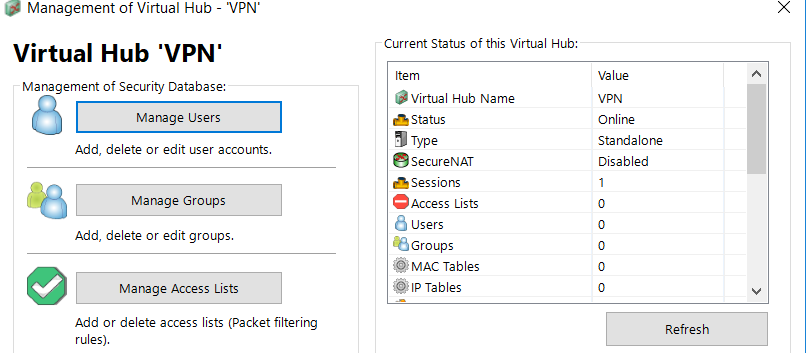
\includegraphics[width=0.6\textwidth]{SoftEther/korak14}
\end{figure}
\FloatBarrier
Na ovom prozoru odabiremo ``Manage Users''.
\begin{figure}[h!]
     \centering
     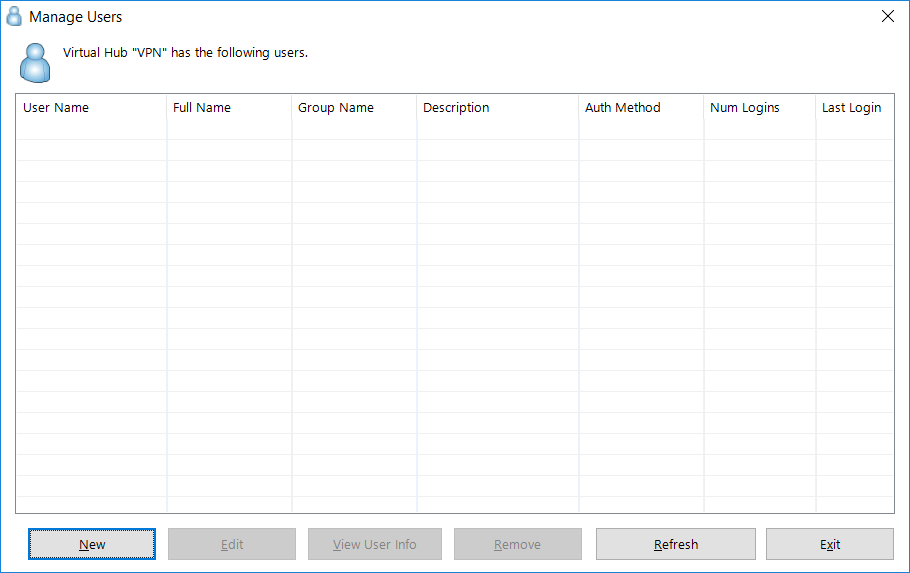
\includegraphics[width=0.4\textwidth]{SoftEther/korak15}
\end{figure}
\FloatBarrier
Sada dodajemo korisnika kojem ćemo dodati proizvoljno ime (u ovim je uputama korisnik nazvan ``klijent1'' i u svim narednim koracima gdje se to ime pojavljuje vama će se pojaviti vaše odabrano ime). Kako bismo smanjili vjerojatnost zlouporabe VPN-a, odabiremo mogućnost prijave klijenta uporabom našeg certifikata i lozinke. Zbog toga odabiremo ``Create Certificate''.
\begin{figure}[h!]
     \centering
     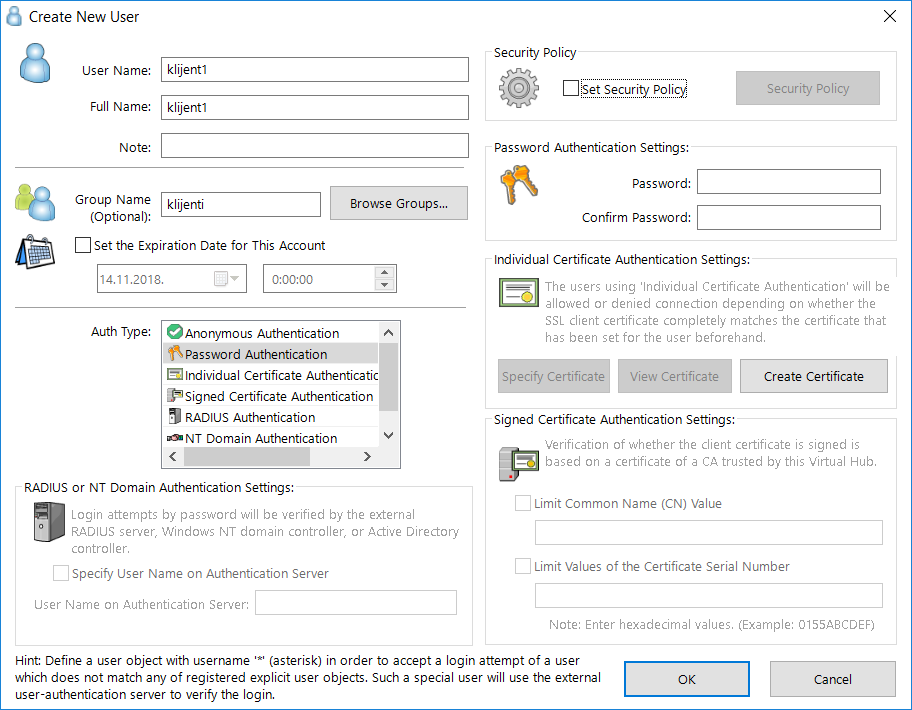
\includegraphics[width=0.6\textwidth]{SoftEther/korak16}
\end{figure}
\FloatBarrier
U sljedećim je poljima moguće detaljno odrediti opis stvorenog klijenta kao i vrijeme njegovog postojanja.
\begin{figure}[h!]
     \centering
     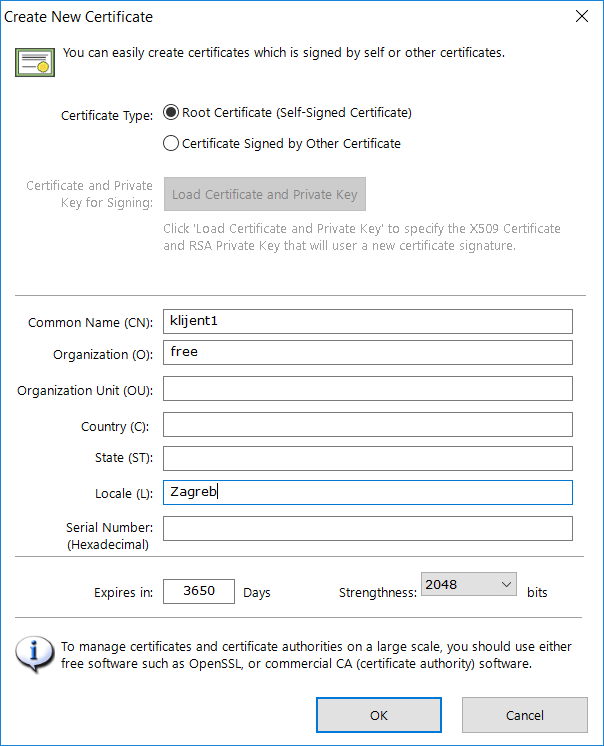
\includegraphics[width=0.6\textwidth]{SoftEther/korak17}
\end{figure}
\FloatBarrier
Nakon otvaranja ovog prozora postavljamo lozinku kojom će se naš klijent prijavljivati na server i koja će samo njemu biti poznata.
\begin{figure}[h!]
     \centering
     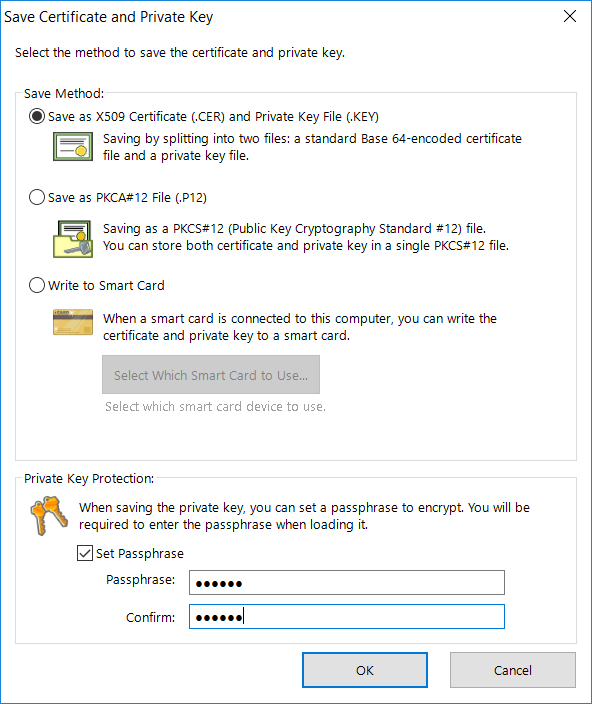
\includegraphics[width=0.6\textwidth]{SoftEther/korak18}
\end{figure}
\FloatBarrier
Nakon potvrde nastaju dvije datoteke: jedna je .cer, a druga je .key i obje su neophodne za prijavu na naš server zato ih mi moramo spremiti i prebaciti na računala koja će se htjeti povezati na server. Povezivanje na server objašnjeno je u jednom od sljedećih dijelova poglavlja.
\begin{figure}[h!]
     \centering
     
\includegraphics[width=0.3\textwidth]{SoftEther/korak20}
\end{figure}
\FloatBarrier
Nakon potvrde vidljiv je korisnik koji se može spojiti na naš server. Moguće je naravno dodavanje više različitih korisnika i brisanje istih.
\begin{figure}[h!]
     \centering
     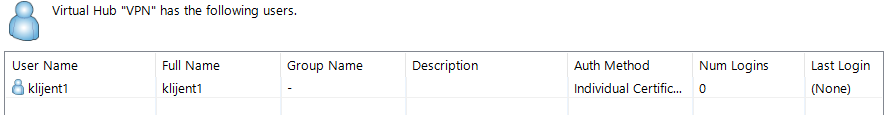
\includegraphics[width=0.6\textwidth]{SoftEther/korak19}
\end{figure}
\FloatBarrier

\newpage
\paragraph*{Instalacija SoftEther klijenta}

\hfill \smallbreak
Za razliku od instalacije i konfiguracije servera, instalacija je SoftEther klijenta jednostavnija. Prvi je korak preuzimanje instalacije sa službene stranice SoftEthera:\\ \url{https://www.softether.org}
\begin{figure}[h!]
	\centering
     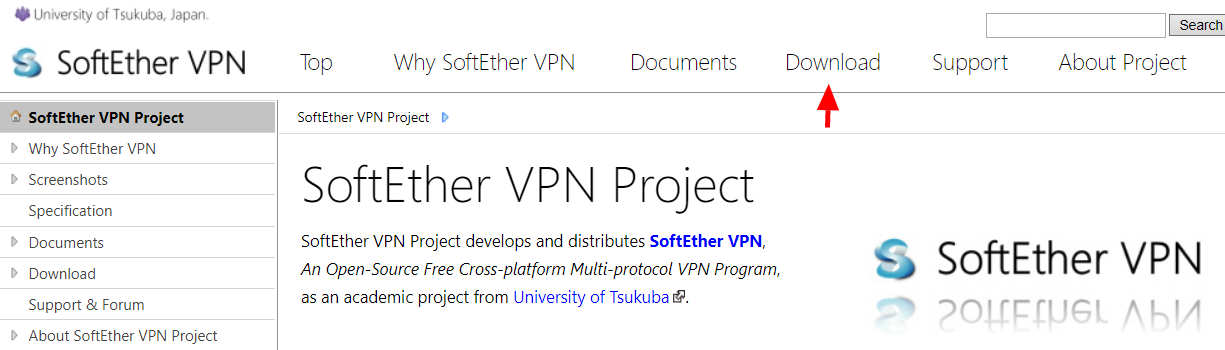
\includegraphics[width=0.6\textwidth]{SoftEther/korak1}
\end{figure}
\FloatBarrier
Odabirom ``Download'' iz izborne trake prikazuje se stranica s ponuđenim poveznicama za preuzimanje.
\begin{figure}[h!]
     \centering
     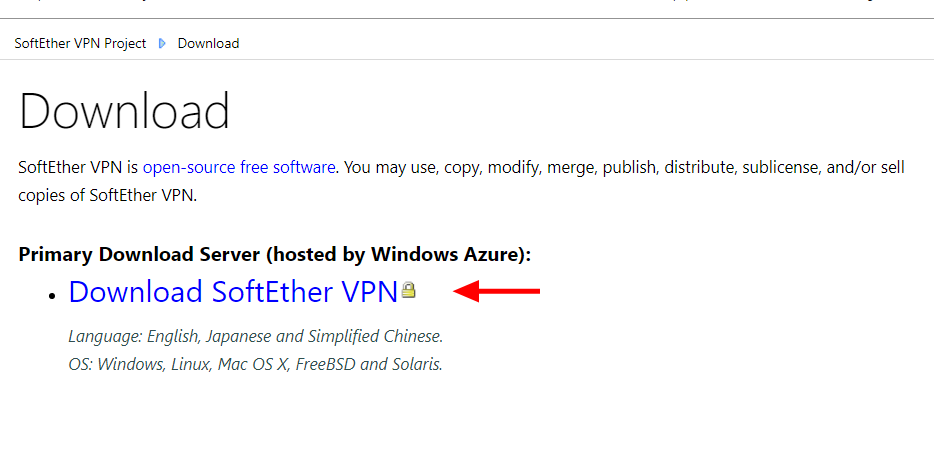
\includegraphics[width=0.6\textwidth]{SoftEther/korak2}
\end{figure}
\FloatBarrier
Sljedeći isječak prikazuje stranicu koja se otvori odabirom prve poveznice. Na stranici se nalaze izborni okviri u kojima je potrebno odabrati željeni program. Za preuzimanje VPN klijenta potrebno je odabrati postavke prikazane na sljedećem isječku te odabrati prvu poveznicu za početak preuzimanja.
\begin{figure}[h!]
     \centering
     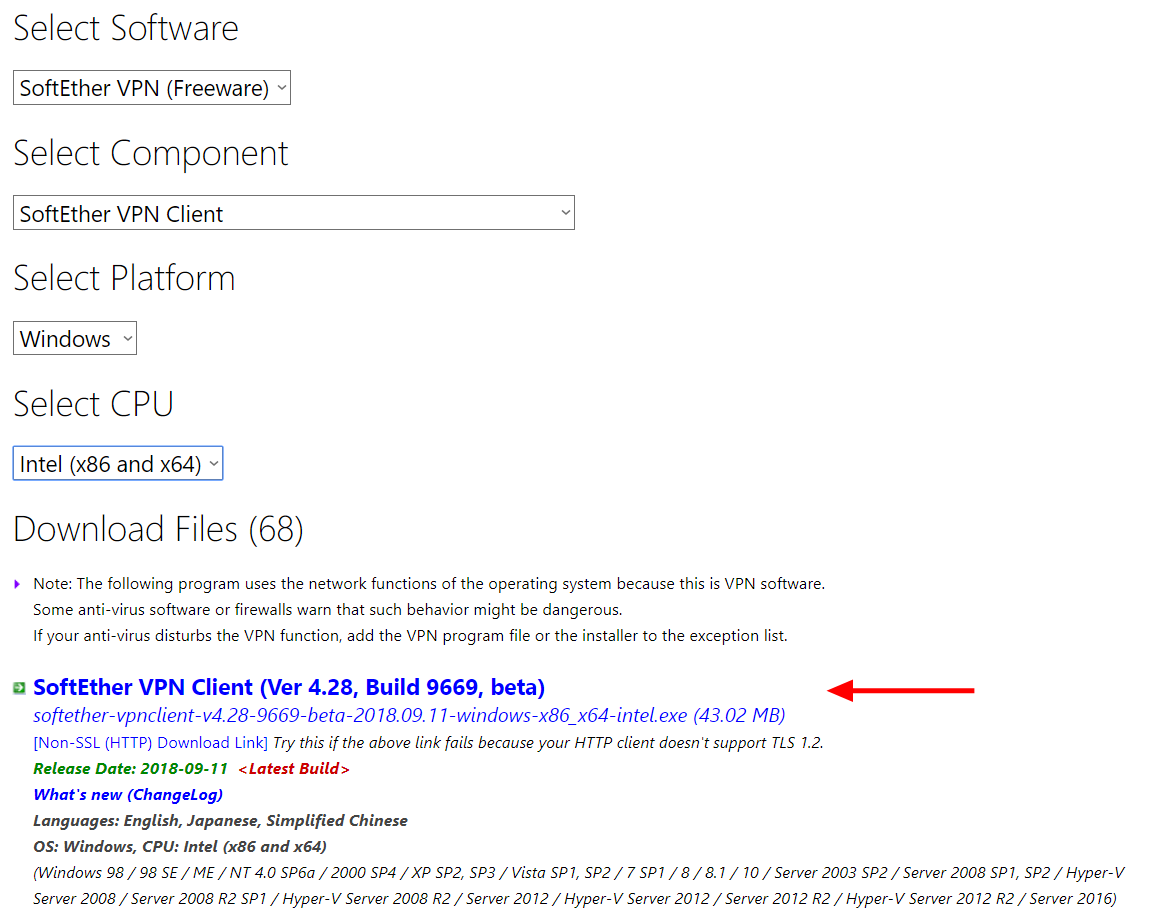
\includegraphics[width=0.6\textwidth]{SoftEther/korak3}
\end{figure}
\FloatBarrier
Nakon završetka preuzimanja i pokretanja instalacije prikazuje se sljedeći prozor. Preporuka je odabrati prvo ponuđeno jer nudi potpunu instalaciju programa.
\begin{figure}[h!]
     \centering
     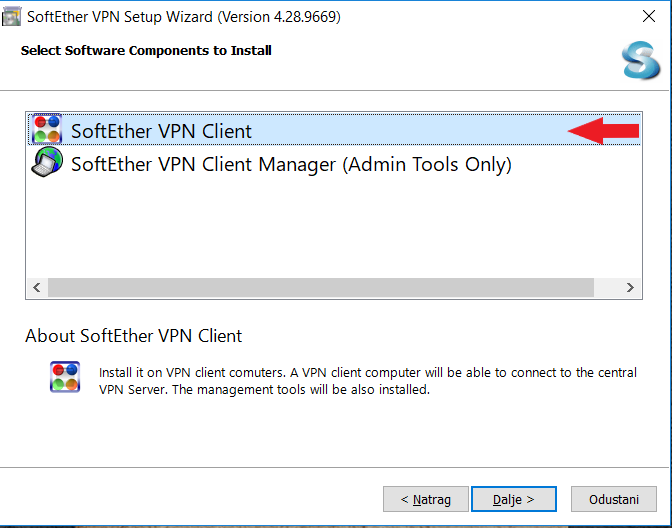
\includegraphics[width=0.6\textwidth]{SoftEther/korak4}
\end{figure}
\FloatBarrier
Ukoliko je instalacija uspješno završena, prikazuje se sljedeći prozor.
\begin{figure}[h!]
     \centering
     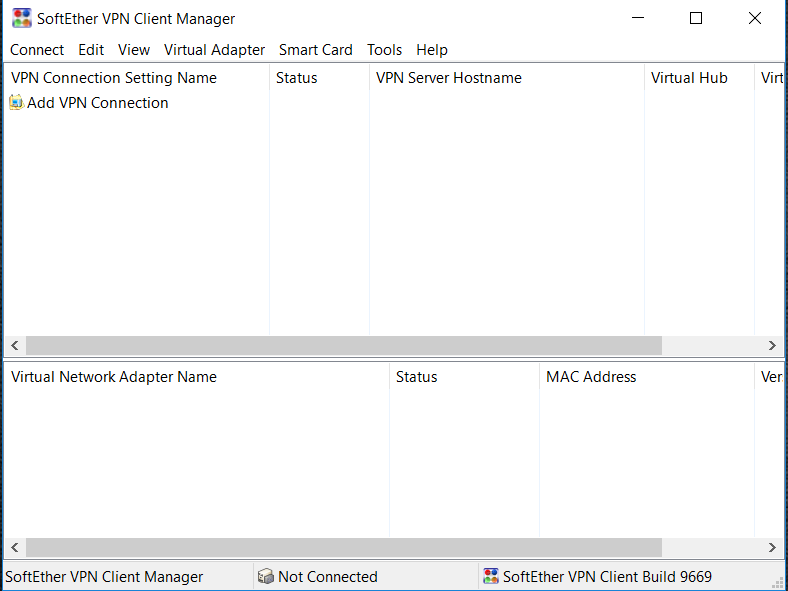
\includegraphics[width=0.6\textwidth]{SoftEther/korak5}
\end{figure}
\FloatBarrier

\newpage
\paragraph*{Povezivanje klijenta sa SoftEther serverom}

\hfill \smallbreak
Za uspješno povezivanje s napravljenim serverom potrebno je pokrenuti aplikaciju SoftEether VPN Client i odabrati opciju dodavanja novog VPN-a. Ako nije postavljen virtualni mrežni adapter, kao što je prikazano u sljedećem primjeru, potrebno je stvoriti novi. Prikazano je stvaranje VPN adaptera.
\begin{figure}[h!]
     \centering
     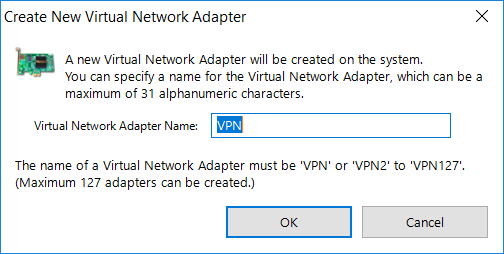
\includegraphics[width=0.6\textwidth]{SoftEther/korak21}
\end{figure}
\FloatBarrier
Nakon stvaranja adaptera moramo dodati server na koji se želimo povezati. Na slici je prikazano stvaranje veze koja se zove VPN. Slično kao i kod stvaranja servera, potrebno je upisati IP adresu preko koje se može serveru pristupiti u polje ``Host name''. Aplikacija nakon upisa IP adrese dohvaća portove na koje se moguće spojiti. Izbor je nekog od ponuđenih portova proizvoljan, kao i postojećih virtualnih mrežnih adaptera. Budući da smo prilikom stvaranja korisnika servera odabrali da se on može prijaviti samo uporabom certifikata i pripadnog ključa, potrebno je stvorene datoteke ``klijent1.cer'' i ``klijent1.key'' prebaciti na računalo s kojeg se pokušava povezati na server. Učitavanje certifikata i ključa u aplikaciju obavlja se odabirom opcije ``specify client certificate''.
\begin{figure}[h!]
     \centering
     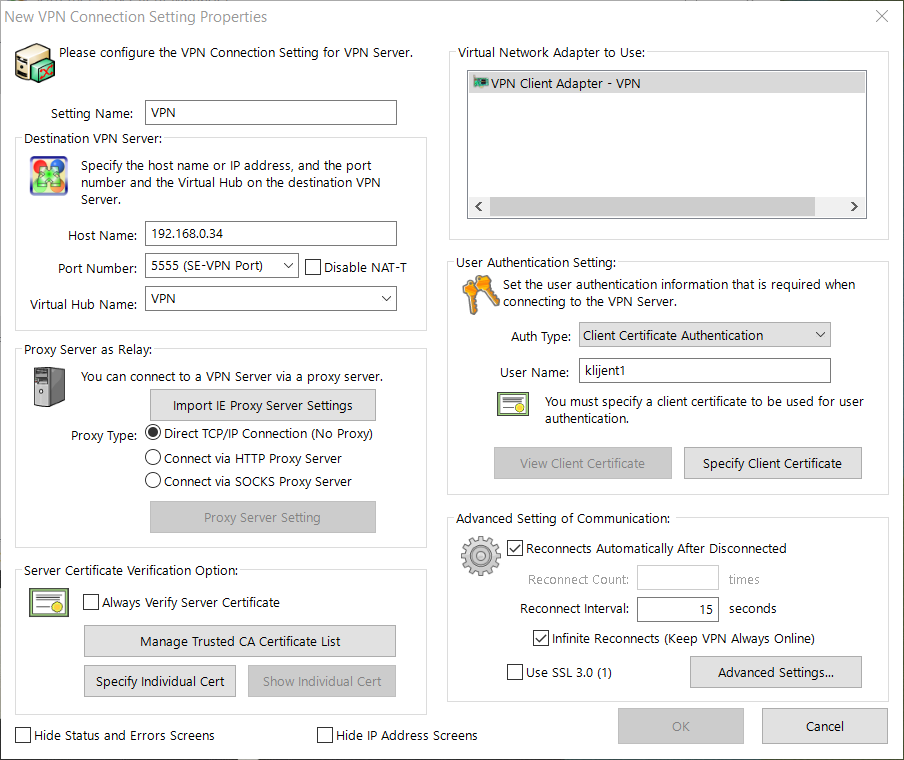
\includegraphics[width=0.6\textwidth]{SoftEther/korak22}
\end{figure}
\FloatBarrier
Nakon učitavanja datoteka prikazuje se prozor sa sljedećeg isječka u koji se upisuje lozinka koju smo postavili prilikom stvaranja klijenta.
\begin{figure}[h!]
     \centering
     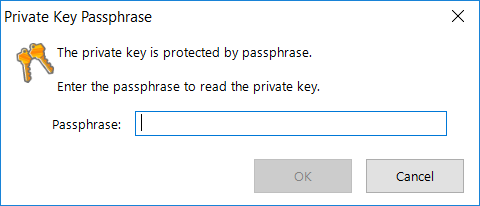
\includegraphics[width=0.6\textwidth]{SoftEther/korak23}
\end{figure}
\FloatBarrier
Ako smo učitali ispravni certifikat i unijeli ispravnu lozinku, tada će se prikazati prozor na kojem vidimo povezivanje s VPN serverom.
\begin{figure}[h!]
     \centering
     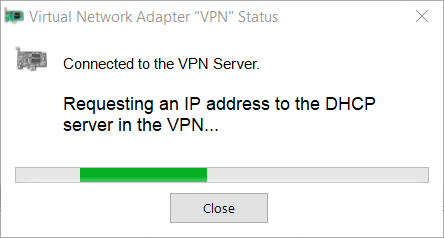
\includegraphics[width=0.5\textwidth]{SoftEther/korak24}
\end{figure}
\FloatBarrier

\FloatBarrier

\subsubsection{Provjera vlastite IP adrese}
\hfill \smallbreak
Kako bi server bio uspješno uspostavljen, potrebna mu je IP adresa dodijeljena računalu na kojem se nalazi. Najbrži način na koji se ona može odrediti jest otvaranje naredbenog retka i upis naredbe IPCONFIG. Rezultat te naredbe bit će prikaz mrežnih postavki za trenutno aktivne mrežne adaptere.
Crvenom je strelicom označena IP adresa na trenutno aktivnom adapteru.
\begin{figure}[h!]
     \centering
     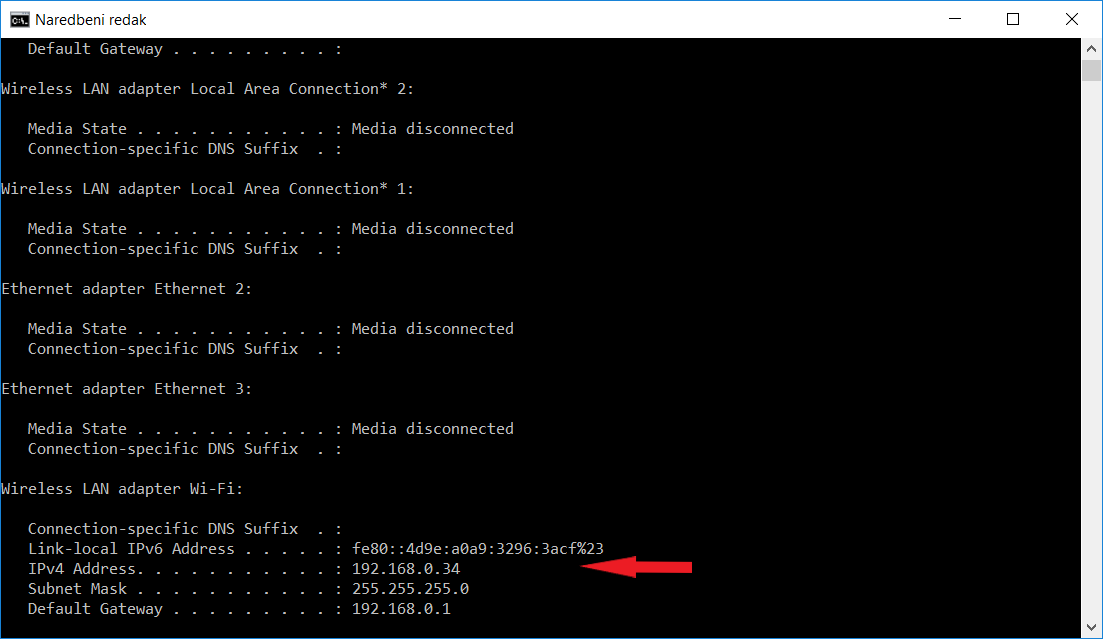
\includegraphics[width=0.6\textwidth]{SoftEther/IP1}
\end{figure}
\FloatBarrier

% za usporedbu === https://www.softether.org/@api/deki/files/12/=1.3.jpg
% pomoć pri instalaciji === https://www.youtube.com/watch?v=VbvRhPqNCsk
	
	\newpage
	\section{FreeBSD}
	\subsection{FreeBSD VPN over IPsec}
	Ovo poglavlje će uključivati postavljanje VPN-a na FreeBSD inačici operacijskog
sustava BSD. 
    Potreban nam je poslužitelj za po mogućnosti sa statičkom IP adresom. Ovdje
    ćemo koristiti platformu DigitalOcean koja omogućuje brzo i jednostavno
    podizanje i upravljanje poslužiteljem. Za pristup poslužitelju koristit ćemo
    ssh protokol za što nam je potreban par ključeva koje generiramo naredbom \\

    \noindent
    \code{\$ ssh-keygen -t rsa -b 2048} \\

    \noindent
    Javni ključ se nalazi u datoteci \code{~/.ssh/id\_rsa.pub}, a privatni, koji
    mora ostati tajan, u \code{~/.ssh/id\_rsa}.

    Nakon registracije na Digital Ocean na svojem profilu možemo dodati javni ključ
    koji ćemo kasnije koristiti za pristup poslužitelju. Sada možemo stvoriti
    poslužitelja. Odabrat ćemo opciju
    \textit{Create Droplet} i odabrati sljedeće postavke:

    \begin{figure}[h]
        \centering
        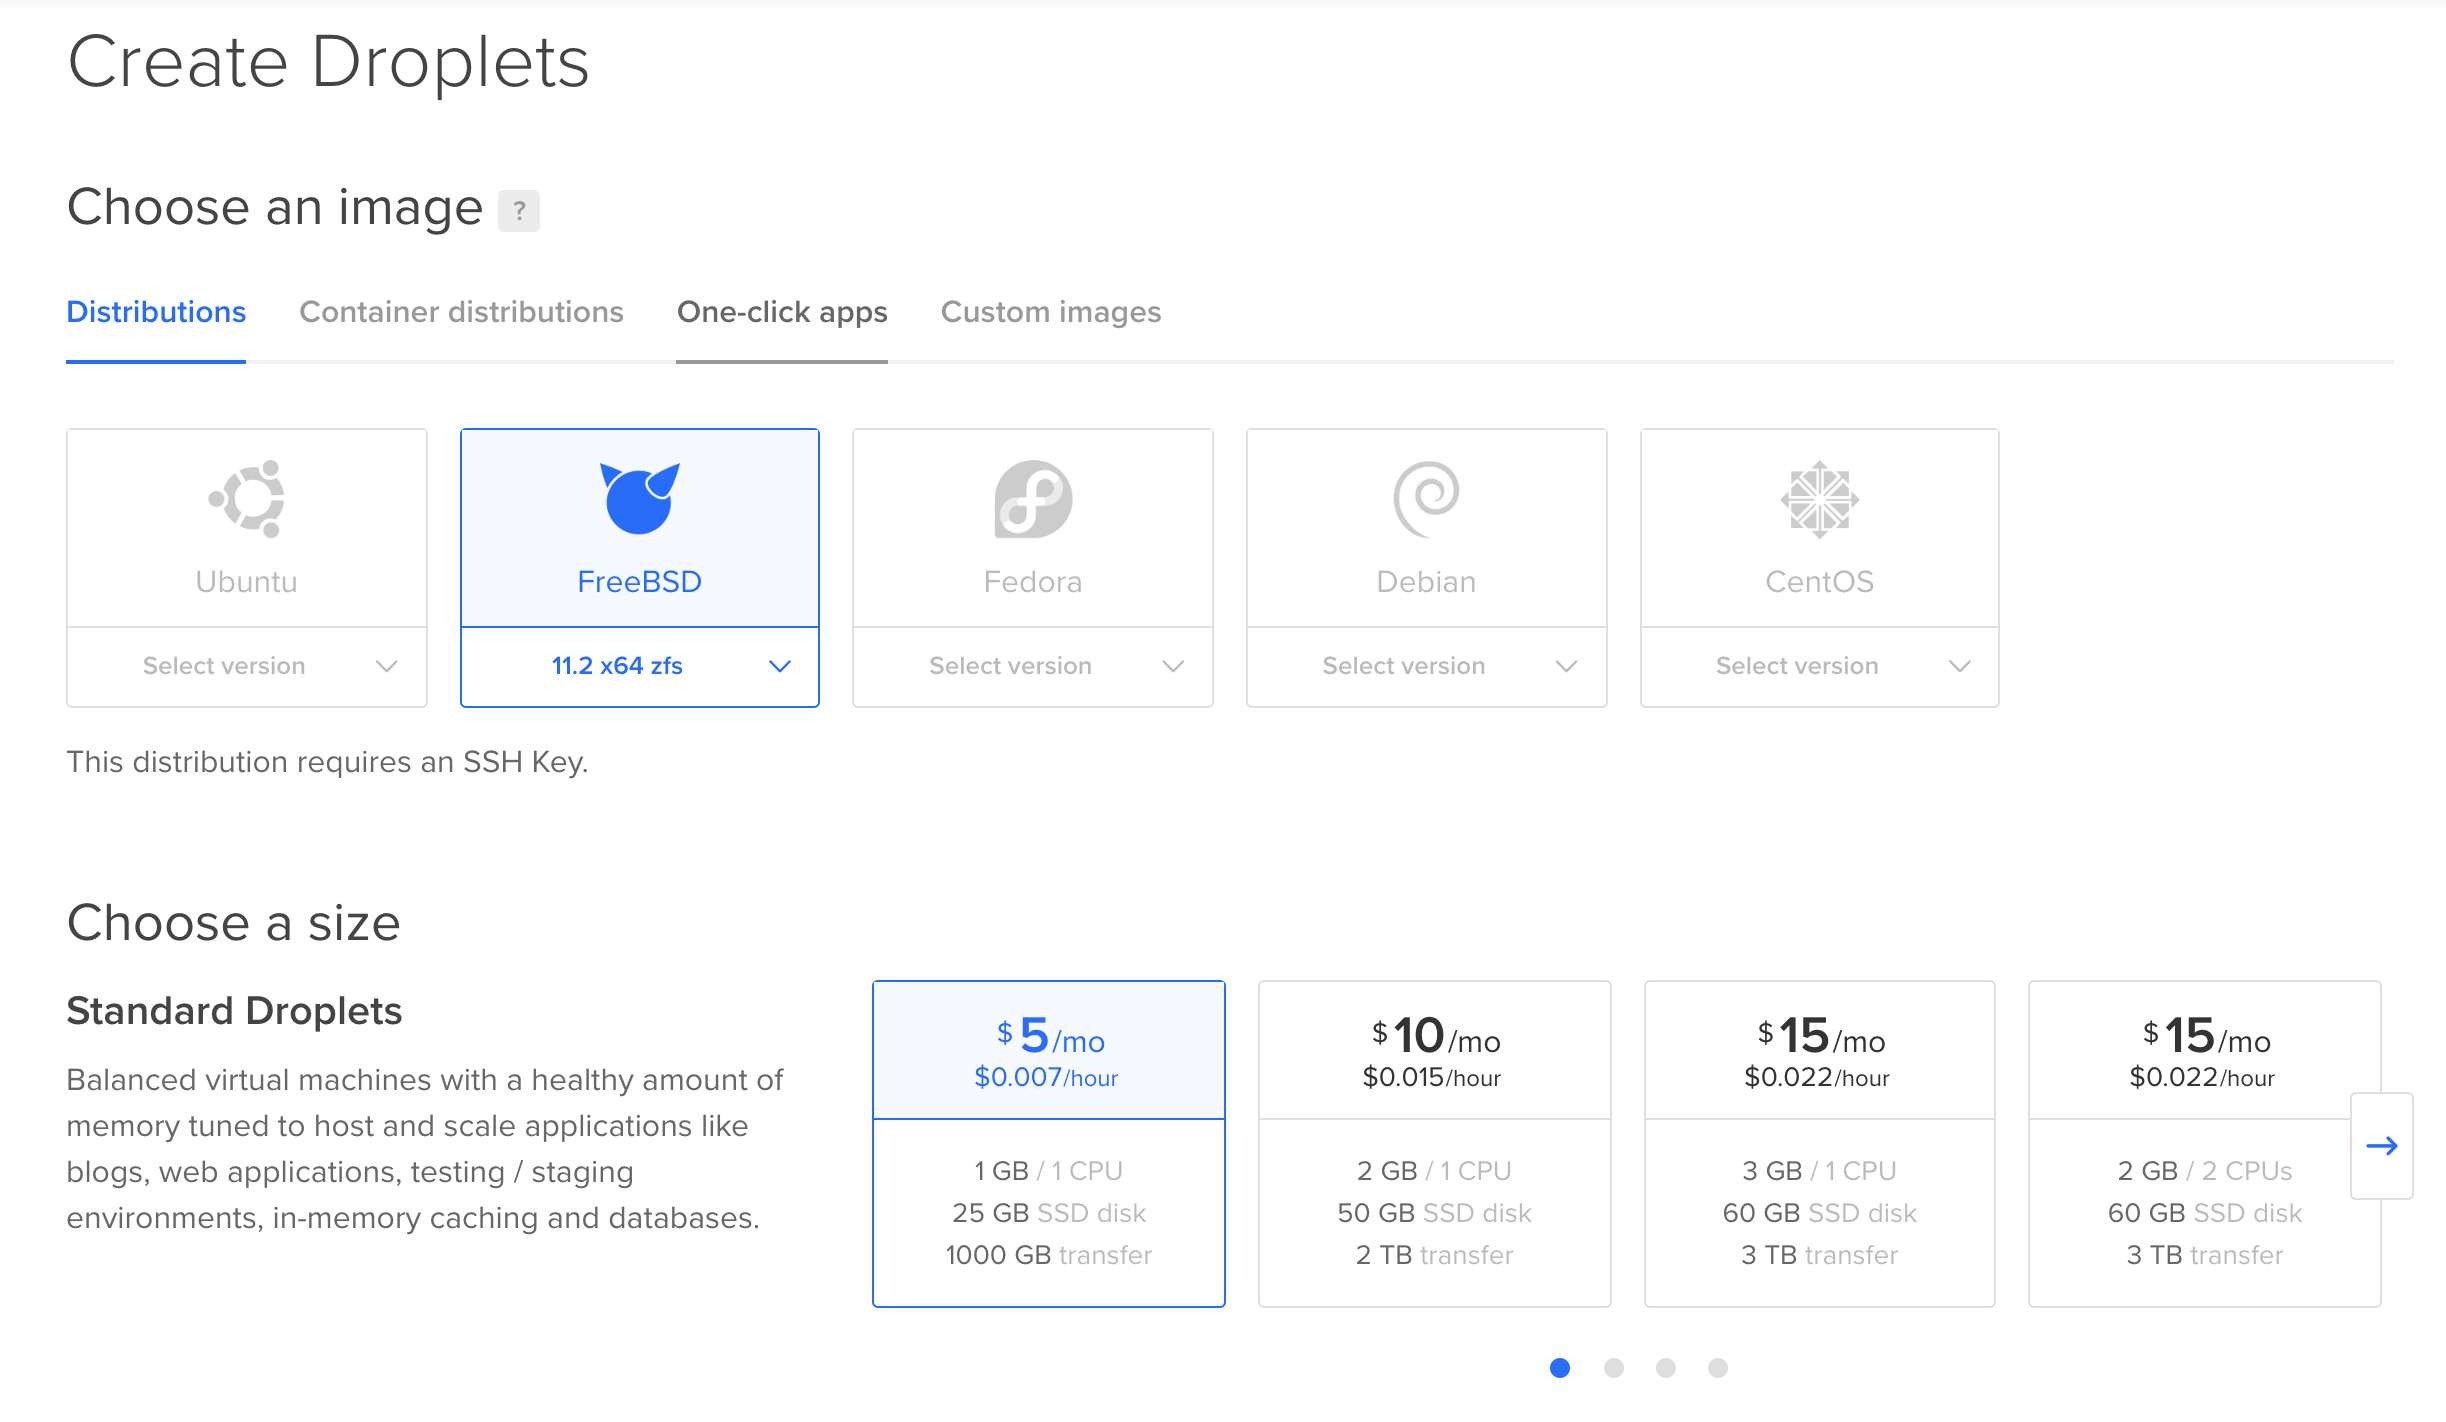
\includegraphics[scale=0.35]{slike/postavkeDOserver}
        \caption{Postavke DigitalOcean poslužitelja}
    \end{figure}

    \newpage
    \noindent
    Digital Ocean nam također nudi opciju da odaberemo lokaciju našeg poslužitelja
    i pripremimo ssh ključeve kako bi si olakšali pristup
    \begin{figure}[h]
        \centering
        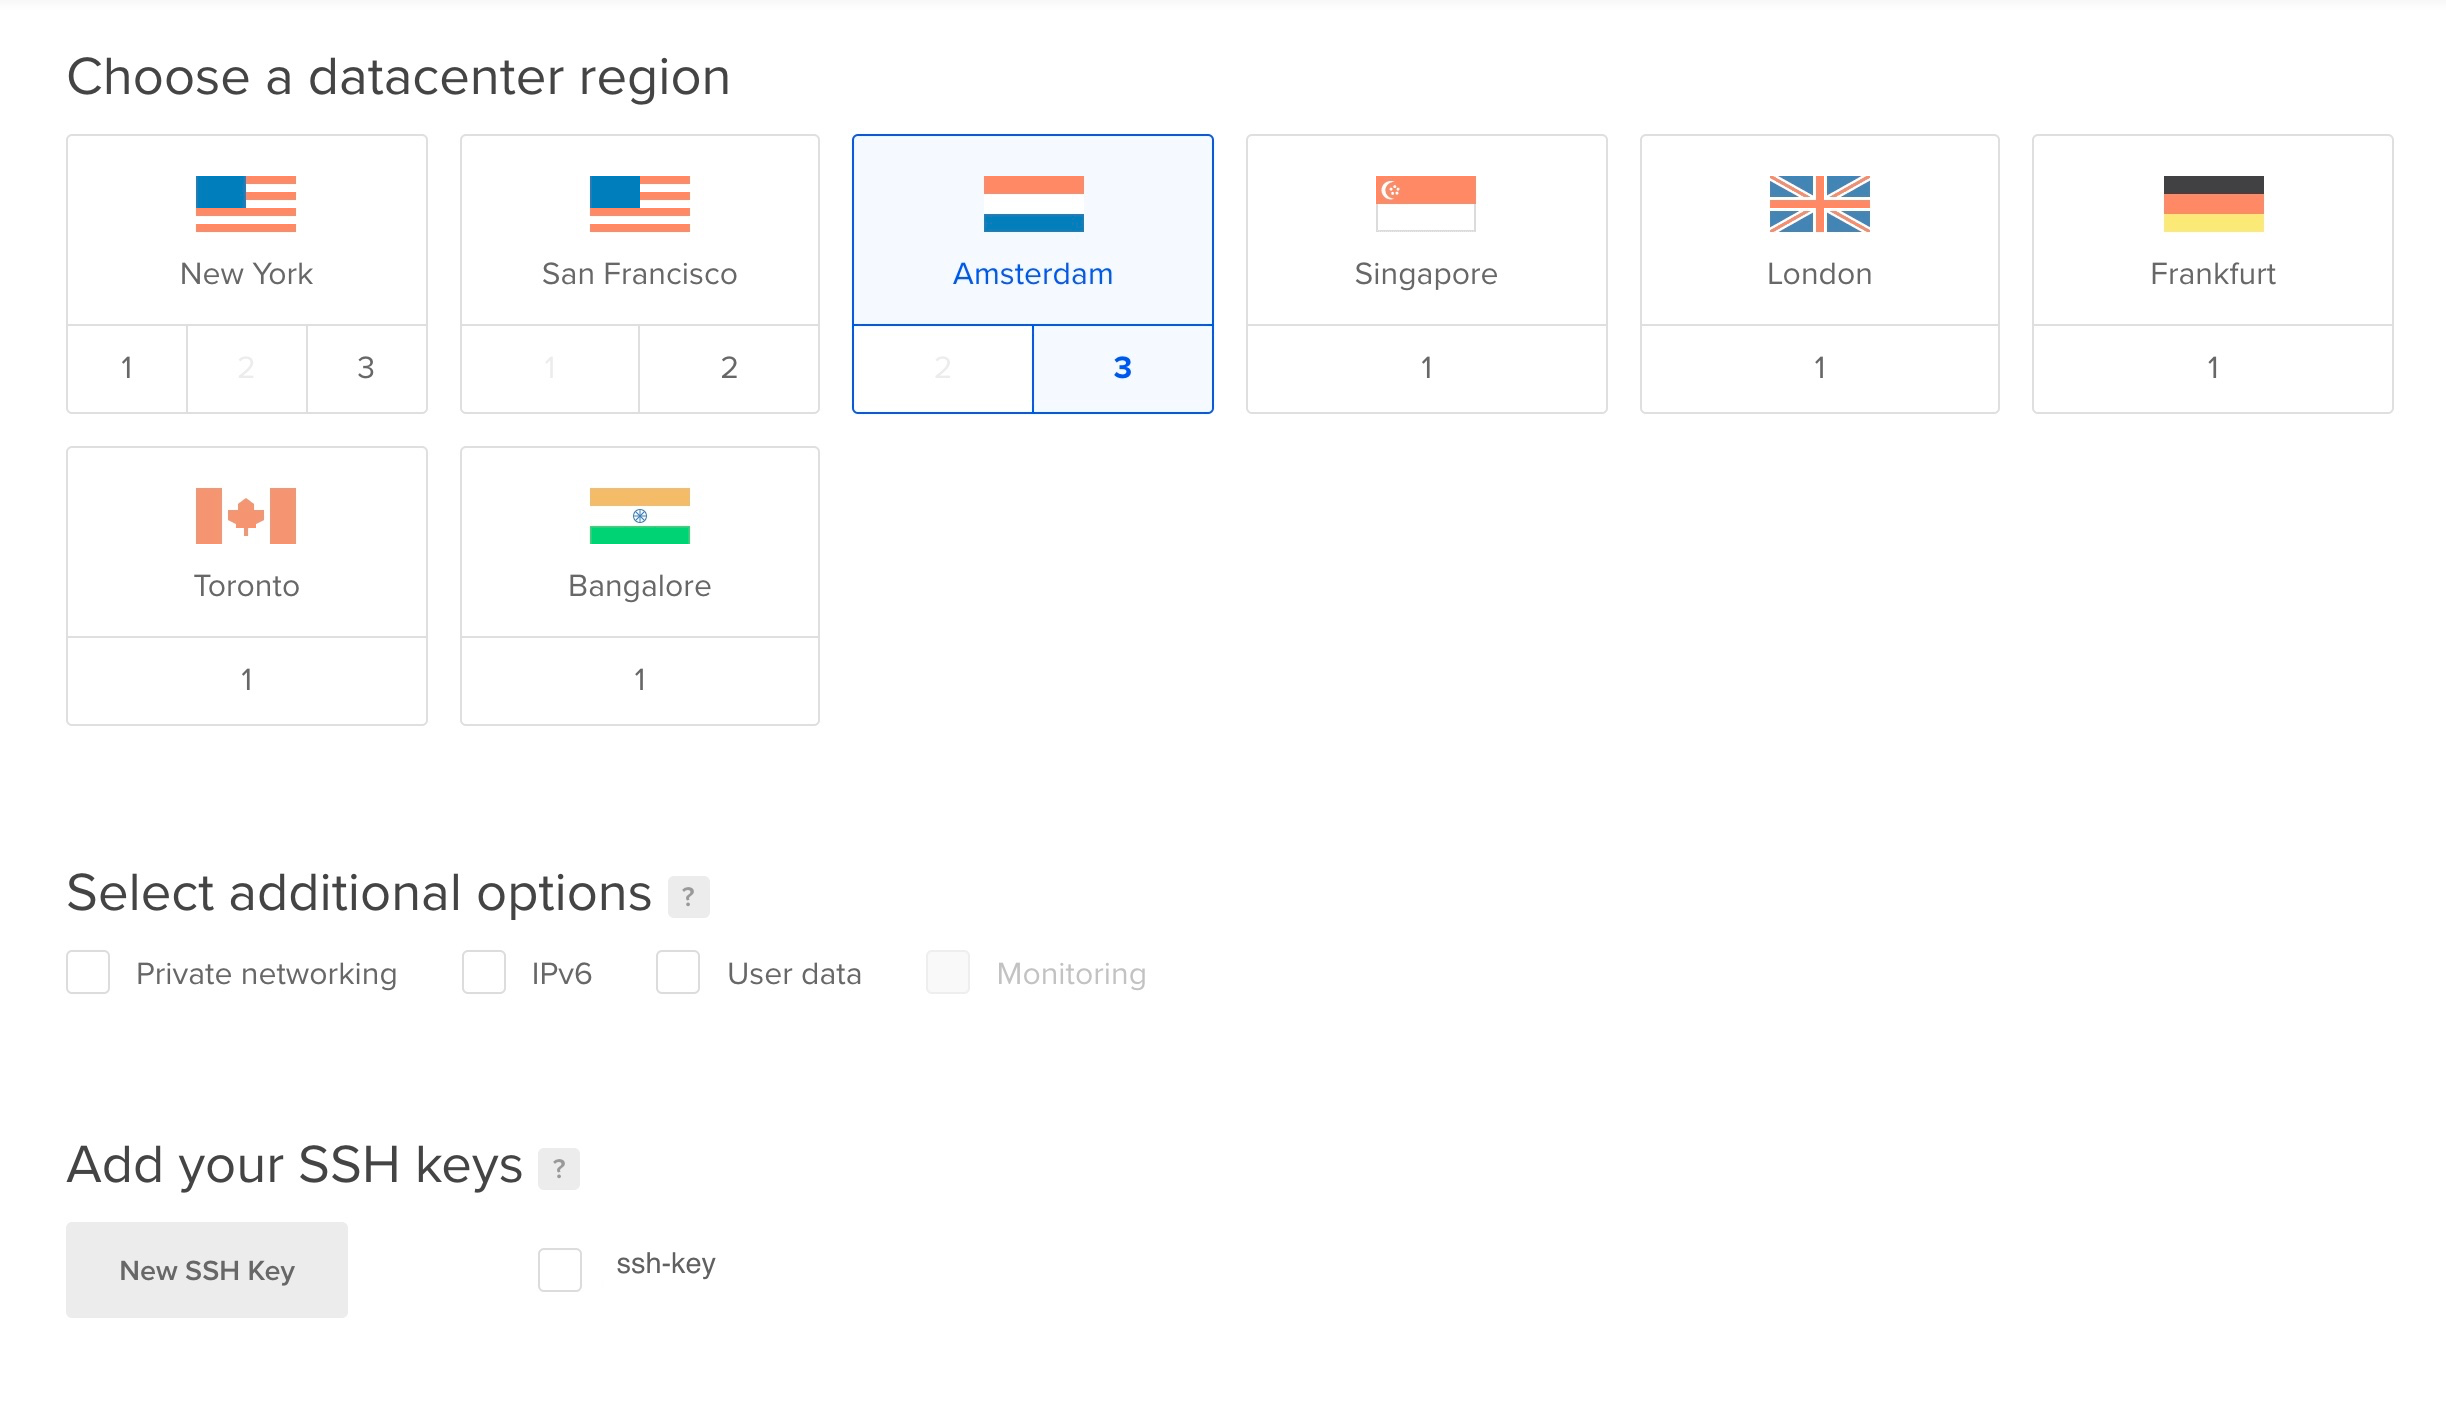
\includegraphics[scale=0.15]{slike/lokacijaIssh}
        \caption{Odabir lokacije i ssh ključeva}
    \end{figure}

    Kako sada prvi puta pristupamo poslužitelju jedini korisnik
    koji postoji je root. Root je korisnik na unixoidima koji može izvršiti
    svaku naredbu i pristupiti svakoj datoteci. Njemu pristupamo naredbom \\
    
    \noindent
    \code{\$ ssh root@139.59.159.111} \\

    Kada smo se prijavili na poslužitelja prvu stvar koju moramo napraviti je
    ažurirati sustav. To ćemo napraviti koristeći FreeBSD-ov upravitelj
    paketima \code{pkg} i njegove naredbe \code{update} i \code{upgrade}. \\

    \noindent
    \code{\# pkg update} \\
    \code{\# pkg upgrade} \\

    Sada možemo instalirati OpenVPN. \\

    \noindent
    \code{\# pkg install openvpn} \\

    Konfiguracijske datoteke ćemo smjestiti u direktorij
    \code{/usr/local/etc/openvpn} koji prvo moramo stvoriti. \\

    \noindent
    \code{\# mkdir /usr/local/etc/openvpn} \\

    \noindent
    Openvpn nudi predloške konfiguracijskih datoteka stoga ćemo kopirati
    predložak za konfiguraciju poslužitelja u naš direktorij

    \noindent
    \code{\# cp
    /usr/local/share/examples/openvpn/sample-config-files/server.conf
    \textbackslash} \\
    \code{\-\ \-\ \-\ \-\ \-\ /usr/local/etc/openvpn/openvpn.conf}

        Kako bi mogli zaštititi našu vezu potrebno je šifrirati sav promet
        između poslužitelja i klijenta i osigurati integritet svake poruke.
        Za šifriranje podataka ćemo koristiti simetrično šifriranje zbog svoje
        brzine, a za to nam je potreban simetrični ključ odnosno više ukoliko
        netko uspije dešifrirati jednu od naših poruka. Kako bi osigurali
        integritet poruka potrebno ih je potpisati i omogućiti provjeru
        potpisa. Ovaj problem ćemo riješiti digitalnim certifikatima koje ćemo
        sami napraviti. OpenVPN dolazi s alatom Easy-RSA koji će nam poslužiti za izgradnju
        infrastrukture javnog ključa (\textit{engl. PKI - public key
        infrastructure}). PKI služi kako bi se javni ključevi povezali s
        pripadajućim osobama ili organizacijama. Proces povezivanja izvršava
        tijelo za certificiranje (\textit{engl. CA - certification authority}.
        CA također potvrđuje pripada li javni ključ osobi navedenoj u
        certifikatu. U praksi se CA nalazi na posebnom računalu, ali kako ovo
        radimo za privatnu uporabu naš CA će se nalaziti na poslužitelju.

        Kako je Easy-RSA omotač oko složene programske knjižnice OpenSSL ona
        nam je jedini preduvjet te ćemo ju instalirati naredbom \\

        \noindent
        \code{\# pkg install openssl} \\

        Nakon toga ćemo kopirati \code{easy-rsa} direktorij u naš direktorij sa svom
        konfiguracijom. \\

        \noindent
        \code{\# cp -r /usr/local/share/easy-rsa
        /usr/local/etc/openvpn/easy-rsa} \\

        Sada ćemo se premjestiti u Easy-RSA direktoriji i urediti njegovu
        konfiguracijsku datoteku \code{vars}. \\

        \noindent
        \code{\# cd /usr/local/etc/openvpn/easy-rsa} \\
        \code{\# vim vars} \\

        U nastavku su navedena polja koja je potrebno izmijeniti:
        
        \noindent
        \code{set\_var EASYRSA\_REQ\_COUNTRY   \-\ "<ZEMLJA>"} \\
        \code{set\_var EASYRSA\_REQ\_PROVINCE  "<ZUPANIJA>"} \\
        \code{set\_var EASYRSA\_REQ\_CITY      \-\ \-\ \-\ \-\ "<GRAD>"} \\
        \code{set\_var EASYRSA\_REQ\_ORG       \-\ \-\ \-\ \-\ \-\ "<ORGANIZACIJA>"} \\
        \code{set\_var EASYRSA\_REQ\_EMAIL     \-\ \-\ \-\ "<EMAIL>"} \\
        \code{set\_var EASYRSA\_REQ\_OU        \-\ \-\ \-\ \-\ \-\ \-\  "<ORGANIZACIJSKA JEDINICA>"} \\
        \code{set\_var EASYRSA\_KEY\_SIZE      \-\ \-\ \-\ \-\ <broj> \# duljina rsa ključa u
        bitovima} \\
        \code{set\_var EASYRSA\_CA\_EXPIRE     \-\ \-\ \-\ <broj> \# trajanje CA ključa u
        danima} \\
        \code{set\_var EASYRSA\_CERT\_EXPIRE   \-\ <broj> \# trajanje certifikata u
        danima} \\

        Kako je \code{easy-rsa} skripta pisana za ljusku sh, dok
        FreeBSD koristi csh potrebno je naredbom \code{sh} 
        pokrenuti sh ljusku. Sada možemo inicijalizirati PKI \\

        \code{\# ./easy-rsa.real init-pki} \\
        
        \begin{figure}[H]
            \centering
            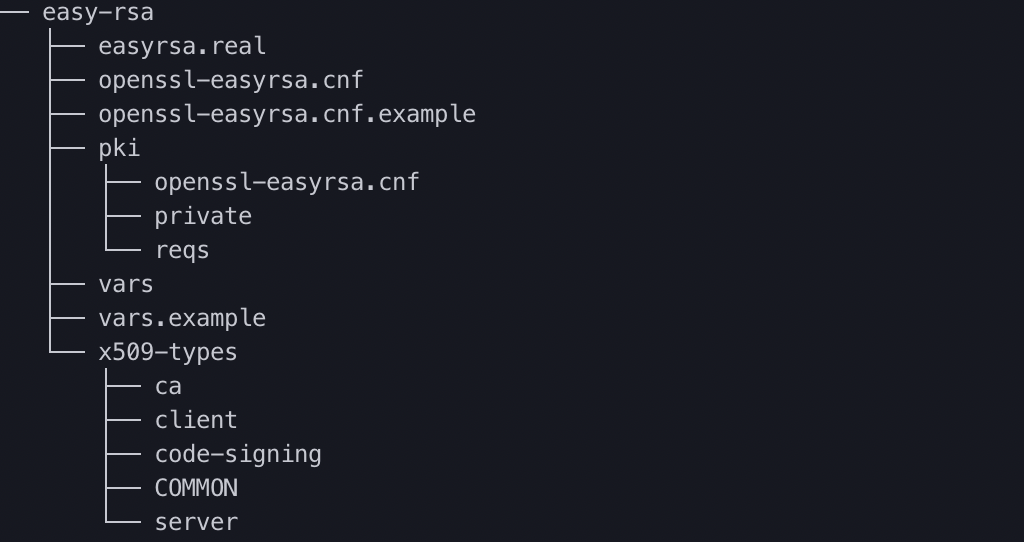
\includegraphics[scale=0.5]{slike/afterPkiInit}
            \caption{Struktura direktorija nakon inicijalizacije PKI}
        \end{figure}
        
        \noindent
        nakon čega ćemo stvoriti CA  \\

        \noindent
        \code{\# ./easy-rsa.real build-ca} \\
        
        \begin{figure}[H]
            \centering
            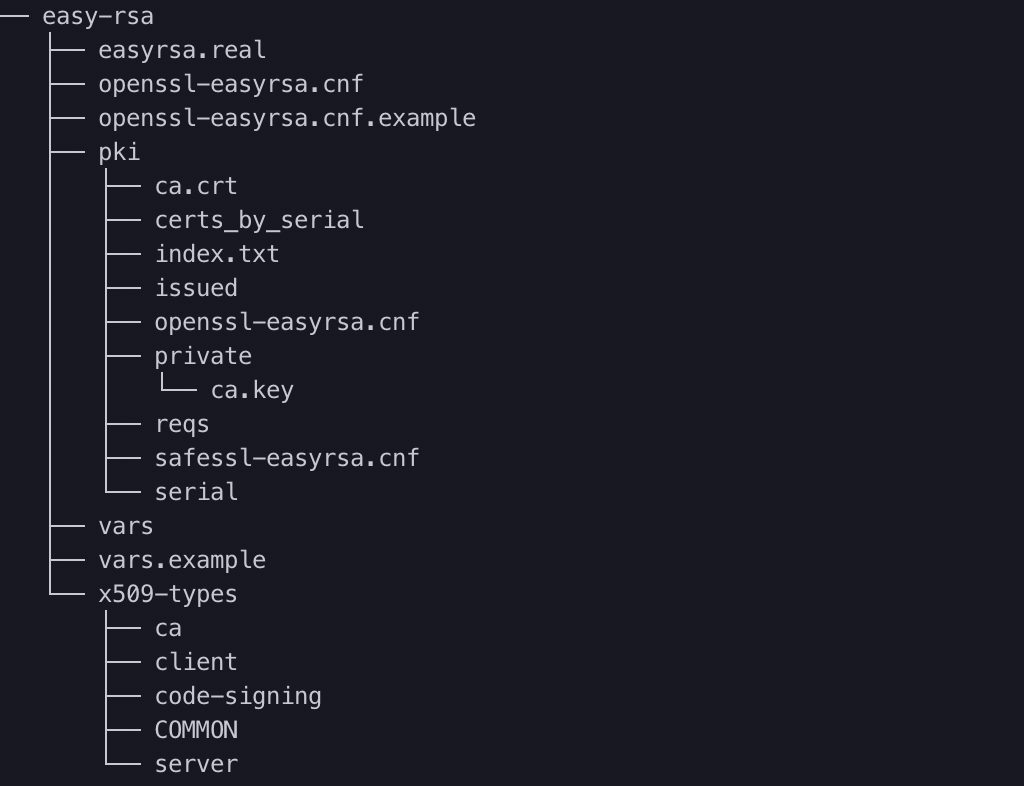
\includegraphics[scale=0.5]{slike/afterBuildCa}
            \caption{Struktura direktorija nakon stvaranja korijenskog
            certifikata}
        \end{figure}

        \noindent
        Ovom naredbom smo stvorili par ključeva koji ćemo koristiti za
        potpisivanje izdanih certifikata. 

        \noindent
        Sada ćemo generirati serverov certifikat naredbom \\

        \noindent
        \code{\# ./easy-rsa.real build-server-full <ime-server> nopass } \\

        \noindent
        gdje je \code{<ime-server>} ime certifikata, a s \code{nopass} opcijom ćemo
        generirati nešifrirani ključ kako bi mogli automatski pokrenuti OpenVPN
        uslugu prilikom pokretanja sustava bez upisivanja lozinke ključa.

        Na sličan način ćemo generirati klijentove certifikate \\

        \noindent
        \code{\# ./easy-rsa.real build-client-full <ime-klijent> nopass} \\
        
        \begin{figure}[H]
            \centering
            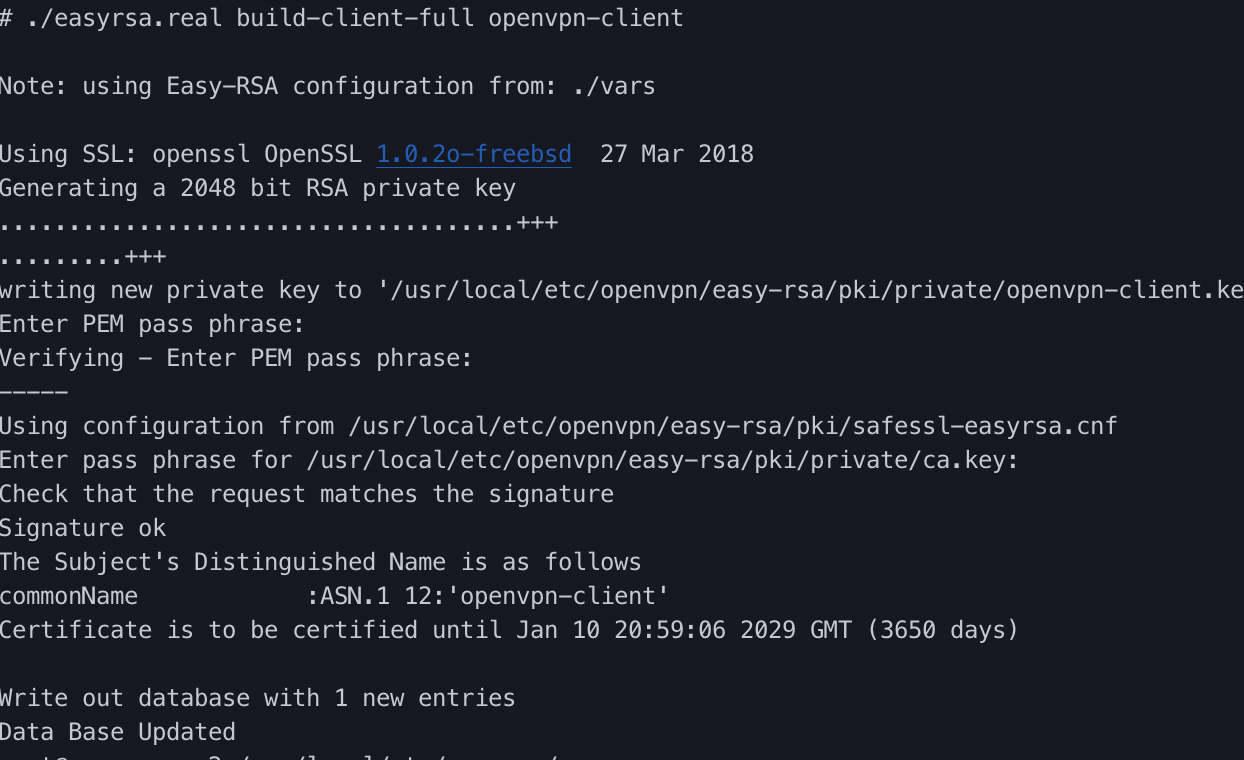
\includegraphics[scale=0.5]{slike/buildClientCert}
            \caption{Stvaranje certifikata}
        \end{figure}

        \begin{figure}[H]
            \centering
            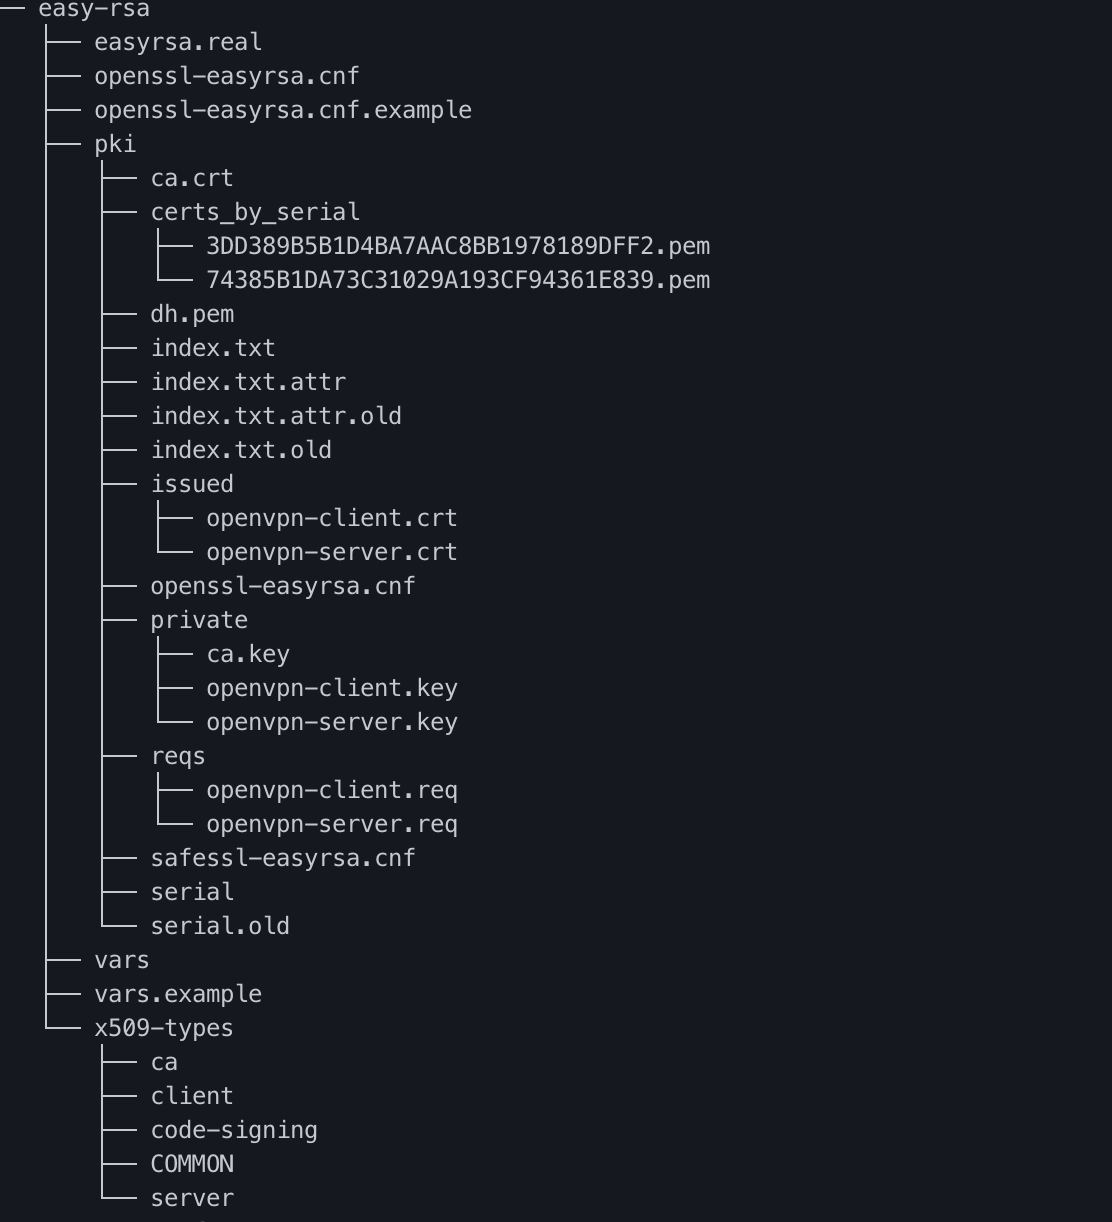
\includegraphics[scale=0.5]{slike/afterClientAndServerCert}
            \caption{Struktura direktorija nakon stvaranja klijentskog i
            poslužiteljevog certifikata}
        \end{figure}

        \noindent
        Za šifriranje same poruke koristit ćemo simetričan ključ generiran
        Diffie-Hellman razmjenom. Za to su nam potrebni Diffie-Hellman
        parametri koje stvaramo naredbom \\

        \noindent
        \code{\# ./easyrsa.real gen-dh} \\


        \noindent
        Do sada smo sve naredbe izvršavali na poslužitelju te smo generirali
        velik broj datoteka od kojih ćemo neke morati premjestiti na klijentsko
        računalo. Kako bi znali koje datoteke premjestiti potrebno je razumjeti
        čemu svaka od njih služi. Sve su datoteke stvorene u
        \code{easy-rsa/pki/} 
        direktoriju pa ćemo se u njega pozicionirati. \\

        \begin{itemize}
        \item \code{ca.crt} - certifikat koji se koristi za validaciju ostalih
        certifikata, potrebno ga je kopirati na poslužitelja i sve klijente
        \item \code{ca.key} - ključ koji CA koristi za izdavanje certifikata
        \item \code{reqs/} - direktorij koji sadrži zahtjeve za izdajom
        certifikata 
        \item \code{issued/<ime-server>.crt} - certifikat servera koji služi za
        provjeru potpisa na poruci, potrebno ga je prebaciti na poslužitelja
        \item \code{private/<ime-server>.key} - privatni ključ poslužitelja
        koji se koristi za potpisivanje poruke, potrebno ga je prebaciti na
        poslužitelja
        \item \code{issued/<ime-klijent>.crt} - certifikat klijenta koji služi za
        provjeru potpisa na poruci, potrebno ga je prebaciti na klijentsko
        računalo
        \item \code{private/<ime-klijent>.key} - privatni ključ klijenta
        koji se koristi za potpisivanje poruke, potrebno ga je prebaciti na
        klijentsko računalo
        \item \code{dh.pem} - Diffie Hellman parametri, potrebno ih je prebaciti na
        poslužitelja
        \end{itemize}

        \noindent
        Ključeve poslužitelja ćemo premjestiti u poseban direktorij \\

        \noindent
        \code{\# mkdir /usr/local/etc/openvpn/keys} \\
        \code{\# cp pki/dh.pem \textbackslash} \\
        \code{\-\ \-\ \-\ \-\ \-\ pki/ca.crt \textbackslash} \\
        \code{\-\ \-\ \-\ \-\ \-\ pki/issued/<ime-server>.crt \textbackslash} \\
        \code{\-\ \-\ \-\ \-\ \-\ pki/private/<ime-server>.key \textbackslash} \\
        \code{\-\ \-\ \-\ \-\ \-\ /usr/local/etc/openvpn/keys} \\

        \begin{figure}[H]
            \centering
            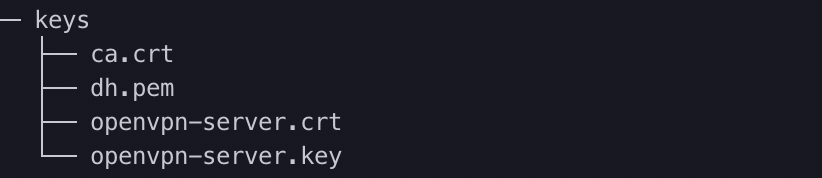
\includegraphics[scale=0.7]{slike/serverKeys}
            \caption{Sadržaj \code{keys} direktorija na poslužitelju}
        \end{figure}

        \noindent
        Prije nego što počnemo konfigurirati klijentsko računalo, potrebno je u
        konfiguraciji poslužitelja navesti putanje do certifikata, ključeva i 
        parametara. To ćemo napraviti u datoteci \code{openvpn.conf} koju smo
        na samom početku kopirali u \code{/usr/local/etc/openvpn}. \\
        
        \noindent
        \code{\# vim /usr/local/etc/openvpn/openvpn.conf} \\
        
        \noindent
        Potrebno je urediti sljedeće linije \\

        \noindent
        \code{ca /usr/local/etc/openvpn/keys/ca.crt} \\
        \code{cert /usr/local/etc/openvpn/keys/<ime-server>.crt} \\
        \code{key /usr/local/etc/openvpn/keys/<ime-server>.key} \\
        \code{dh /usr/local/etc/openvpn/keys/dh.pem} \\ 

        \begin{figure}[H]
            \centering
            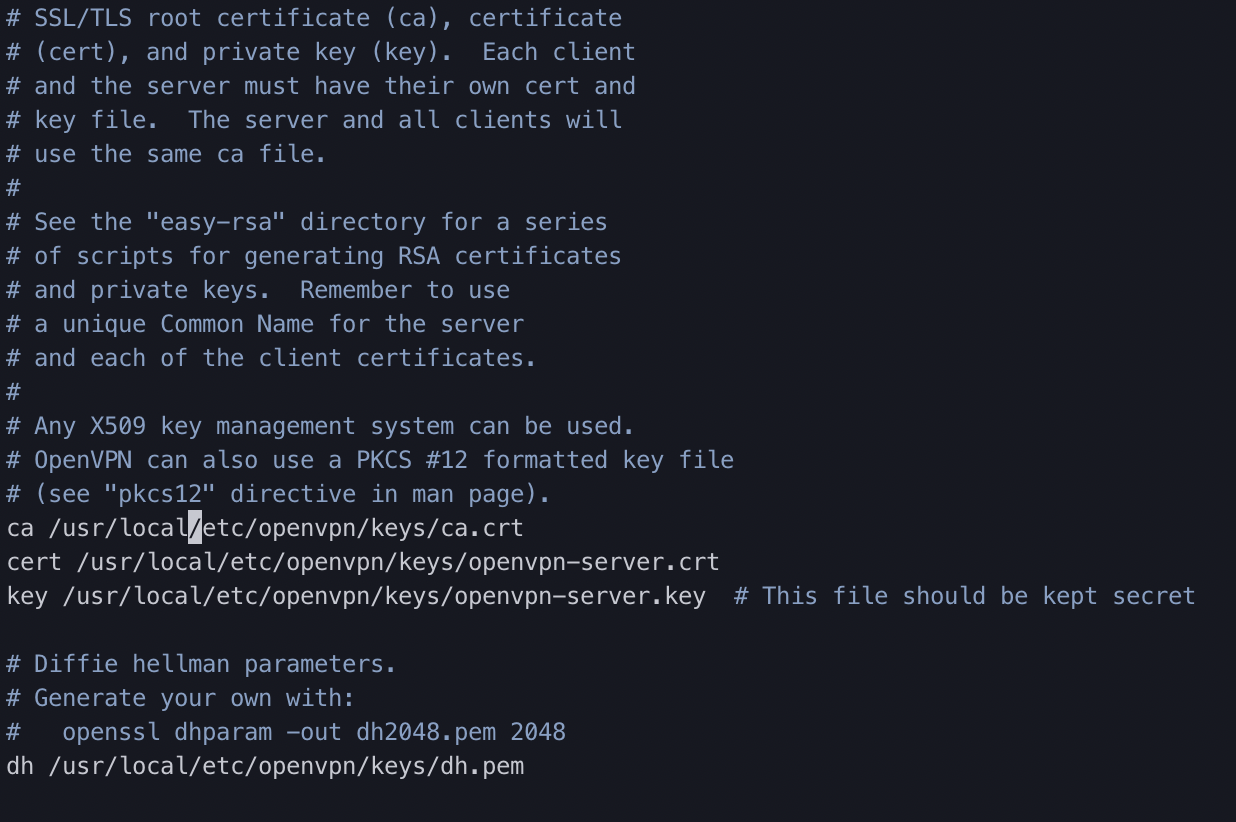
\includegraphics[scale=0.57]{slike/serverPaths}
            \caption{Putanje do ključeva i certifikata u datoteci
            \code{openvpn.conf}}
        \end{figure}
        
        Sada možemo postaviti klijentsko računalo. Kako smo već pripremili
        većinu klijentovih datoteka na poslužitelju, potrebno ih je kopirati.
        Radi se o osjetljivim datotekama stoga nam je potreban siguran način
        slanja datoteka preko mreže za što ćemo koristiti program
        \textit{secure copy}. Nakon što instaliramo openvpn isto kao i na
        poslužiteljskom računalu možemo kopirati predložak konfiguracije \\

        \noindent
        \code{\# cp
        /usr/local/share/examles/openvpn/sample-config-files/client.config
        \textbackslash} \\
        \code{\-\ \-\ \-\ \-\ \-\ /usr/local/etc/openvpn/openvpn.conf} \\

        \noindent
        Također stvorit ćemo direktorij u koji ćemo spremiti ključeve i
        certifikate \\

        \noindent
        \code{\# mkdir /usr/local/etc/openvpn/keys}\\

        \noindent
        Sada možemo kopirati potrebne datoteke s poslužitelja \\

        \noindent
        \code{\$ scp
        root@<ip-server>:/usr/local/etc/openvpn/easy-rsa/pki/ca.crt keys } \\
        \code{\$ scp
        root@<ip-server>:\textbackslash} \\
        \code{\-\
        \-\ \-\ \-\ \-\ \-\ /usr/local/etc/openvpn/easy-rsa/pki/issued/<ime-klijent>.crt
        \textbackslash} \\
        \code{\-\ \-\ \-\ \-\ \-\ \-\ keys} \\
        \code{\$ scp
        root@<ip-server>:\textbackslash} \\
        \code{\-\
        \-\ \-\ \-\ \-\ \-\
        /usr/local/etc/openvpn/easy-rsa/pki/private/<ime-klijent>.key
        \textbackslash} \\
        \code{\-\ \-\ \-\ \-\ \-\ \-\ keys} \\

        \begin{figure}[H]
            \centering
            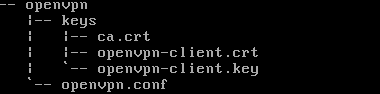
\includegraphics[scale=0.7]{slike/clientKeys}
            \caption{Sadržaj \code{keys} direktorija na klijentu}
        \end{figure}

        \noindent
        U konfiguraciji (\code{openvpn.conf}) osim putanja do certifikata i
        ključeva potrebno je unijeti ip adresu poslužitelja \\

        \noindent
        \code{remote <ip-server> 1194} \\
        \code{ca /usr/local/etc/openvpn/keys/ca.crt} \\
        \code{cert /usr/local/etc/openvpn/keys/<ime-server>.crt} \\
        \code{key /usr/local/etc/openvpn/keys/<ime-server>.key} \\

        Za upravljanje servisima koristimo naredbu \code{service}. Prvo ćemo
        njome pokrenuti OpenVPN servis na poslužitelju i nakon toga na klijentu

        \noindent
        \code{\# service openvpn run} \\

        \noindent
        Sada možemo alatom \code{ifconfig} provjeriti stanje mrežnih sučelja \\
        na klijentu: \\
        \begin{figure}[H]
            \centering
            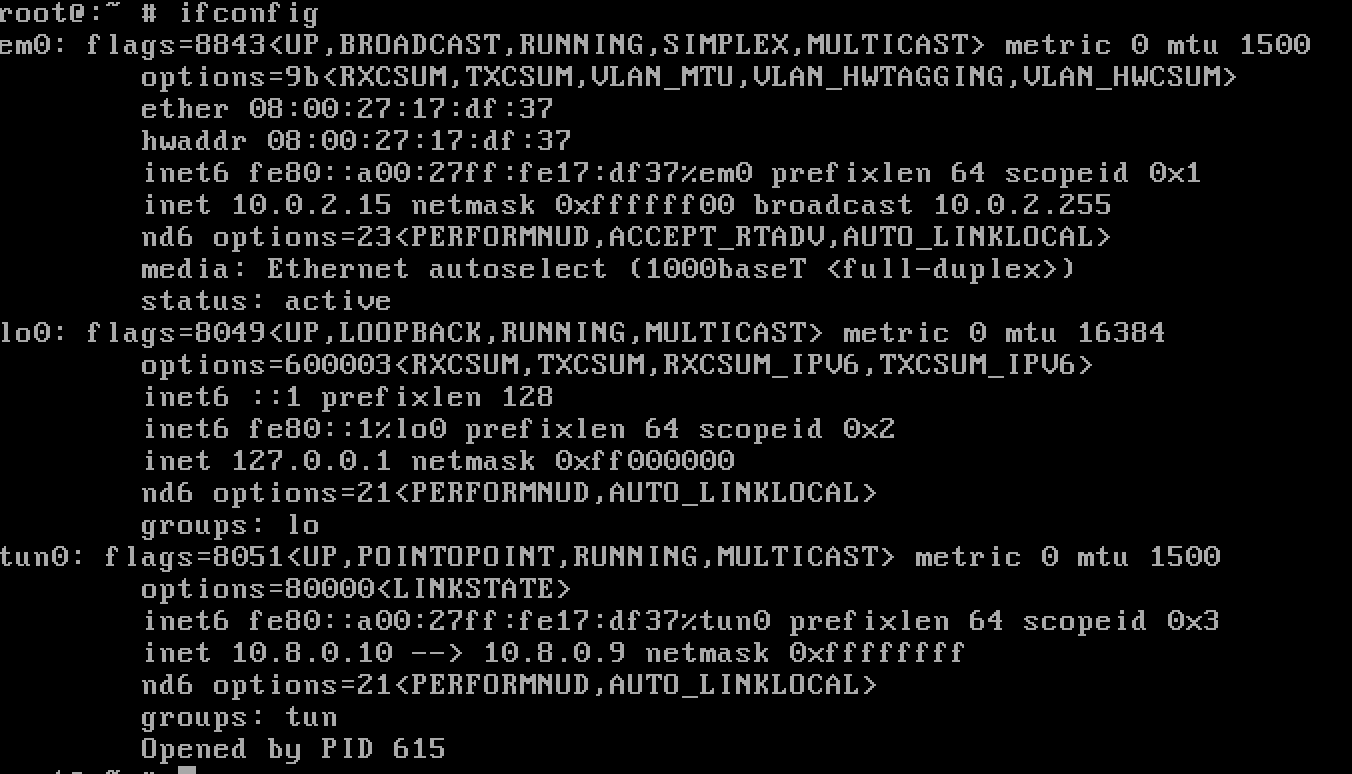
\includegraphics[scale=0.5]{slike/clientIfconfig}
            \caption{Mrežna sučelja klijenta }
        \end{figure}
        na poslužitelju: \\
        \begin{figure}[H]
            \centering
            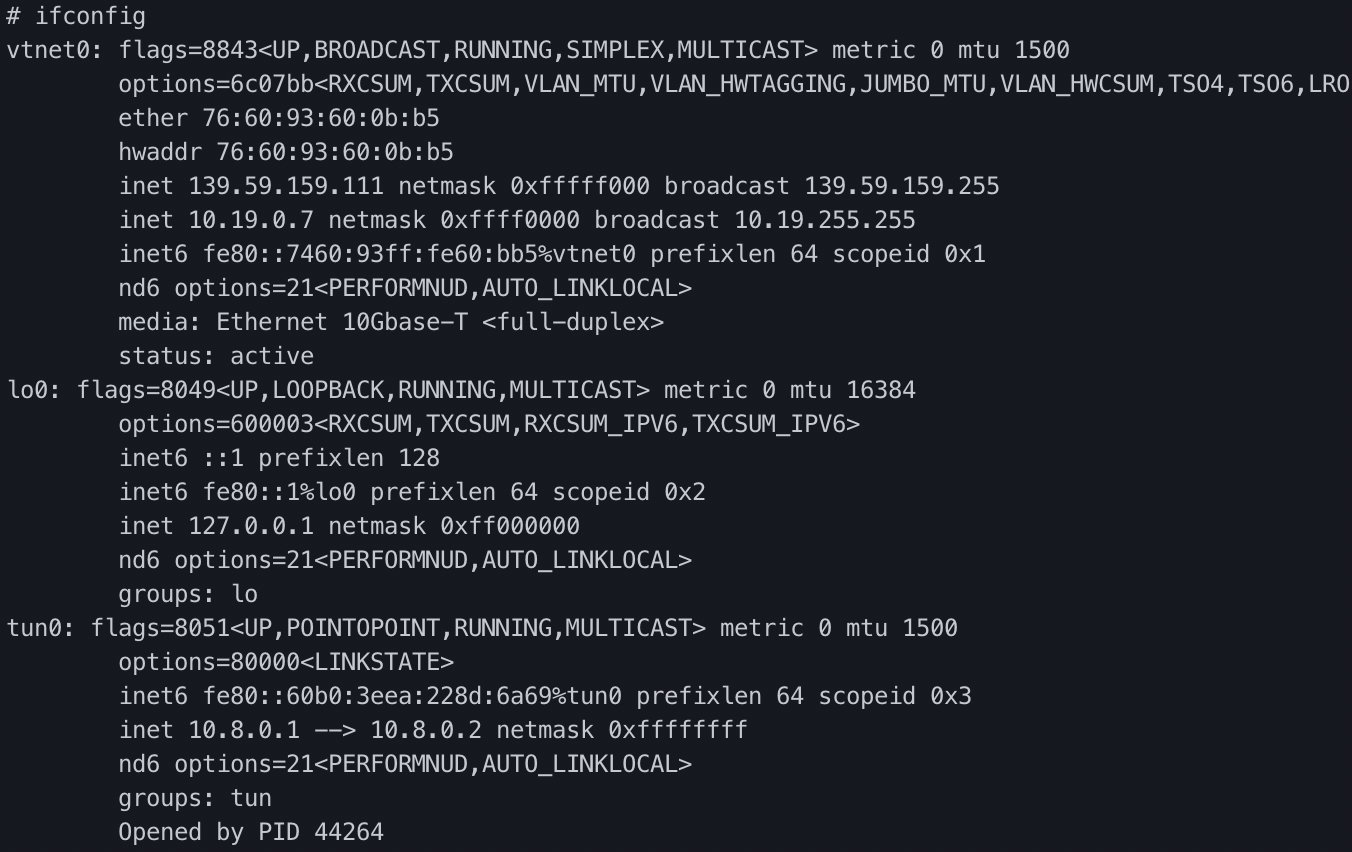
\includegraphics[scale=0.5]{slike/serverIfconfig}
            \caption{Mrežna sučelja poslužitelja}
        \end{figure}

        Možemo uočiti novo sučelje \code{tun0} koje predstavlja virtualno
        sučelje mrežnog sloja. Izvršavanjem naredbe \code{ping} možemo provjeriti je
        li klijentsko računalo stvarno povezano s poslužiteljem. \\

        \noindent
        \code{\$ ping 10.8.0.1} \\

        Kako nam je cilj povezati dva klijenta koji se nalaze u različitim
        privatnim mrežama na isti ćemo pripremiti još jednog klijenta. Njegova
        konfiguracija će biti jednaka konfiguraciji prvog klijenta, a izlaz
        naredbe \code{ifconfig}:
        \begin{figure}[H]
            \centering
            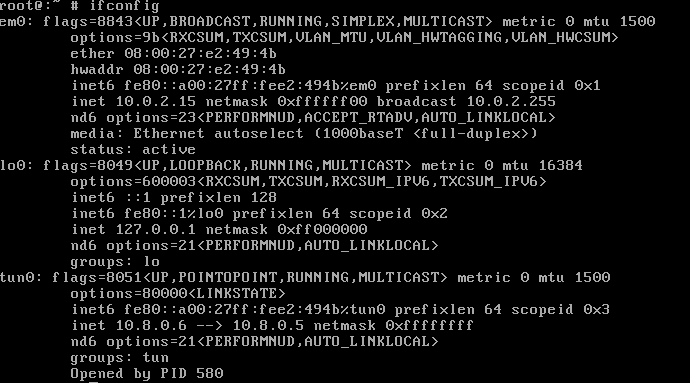
\includegraphics[scale=0.45]{slike/client2Ifconfig}
            \caption{Mrežna sučelja drugog klijenta}
        \end{figure}

        \noindent
        Ako sada pokušamo naredbom
        \code{\$ ping 10.8.0.6}
        provjeriti jesu li klijenti međusobno povezani nećemo dobiti nikakav
        rezultat. Razlog tome je što pretpostavljena konfiguracija poslužitelja
        ne dozvoljava komunikaciju između klijenata. Kako bi to omogućili
        potrebno je u konfiguracijskoj datoteci poslužitelja otkomentirati liniju 

        \noindent 
        \code{client-to-client} \\

        \noindent
        Sada ćemo ponovo pokrenuti OpenVPN i ispitati jesu li klijenti
        međusobno povezani \\

        \noindent
        \code{\# service openvpn restart} \\
        \code{\$ ping 10.8.0.6} \\
        \begin{figure}[H]
            \centering
            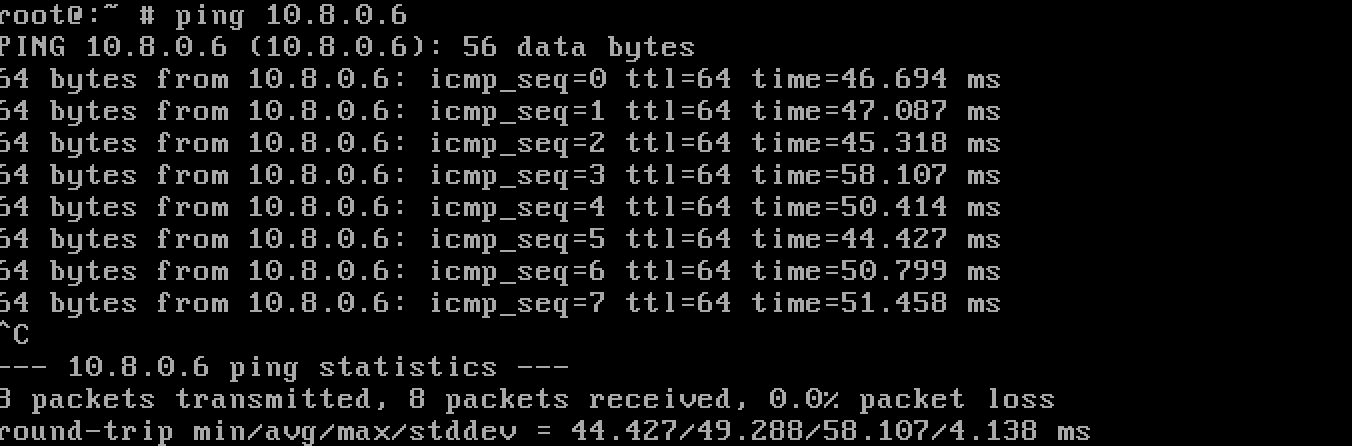
\includegraphics[scale=0.5]{slike/pingResult}
            \caption{Izlaz naredbe ping}
        \end{figure}

        Za kraj možemo pokušati kopirati datoteku s jednog klijenta na drugi
        koristeći \code{tun0} sučelja. Na klijentu s adresom \code{10.8.0.6}
        stvorit ćemo datoteku \code{pozdrav.txt} i u nju nešto zapisati \\ 

        \noindent
        \code{\$ touch pozdrav.txt} \\
        \code{\$ echo "Bok" > pozdrav.txt} \\

        \noindent
        Sada ćemo s drugog klijenta (adresa \code{10.8.0.10}) kopirati
        \code{pozdrav.txt} datoteku i ispisati ju \\
        \code{\$ scp root@10.8.0.6:/root/pozdrav.txt .} \\
        \code{\$ cat /root/pozdrav.txt}\\

        \begin{figure}[H]
            \centering
            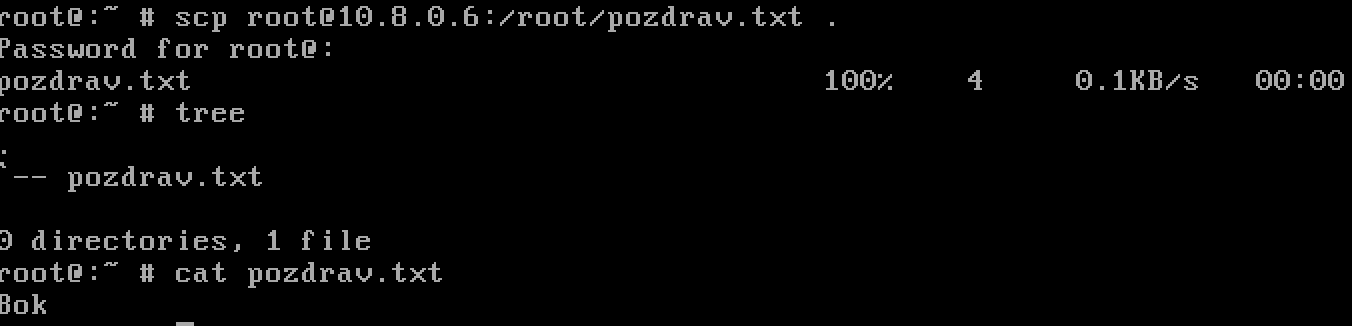
\includegraphics[scale=0.45]{slike/pozdrav}
            \caption{Kopiranje i ispis datoteke \code{pozdrav.txt}}
        \end{figure}


	\newpage
	\section{Linux}
	\subsection{OpenVPN za Ubuntu distribuciju Linux operacijskog sustava}
	

\lstset{
	escapeinside={(*@}{@*)}
}

\bigbreak
\paragraph*{Što je OpenVPN?}
\hfill \smallbreak
OpenVPN\cite{openvpn} je potpuno otvoreni kod za SSL VPN soluciju koji zastupa širok raspon različitih konfiguracija, pritom uključujući udaljeni pristup, \textit{site-to-site} VPN-ove, sigurnost Wi-Fi-a te nudi rješenja za udaljeni pristup prilagođen profesionalnim okruženjima. Sigurnosni model OpenVPN-a bazira se na protokolima SSL/TLS, koji su industrijski standard za sigurnu komunikaciju preko interneta.

\bigbreak
\paragraph*{Prije početka instalacije}
\hfill \smallbreak
 Ove upute\cite{tutorialopenvpn} prilagođene su za verziju 16.04 Ubuntu distribucije operacijskog sustava Linux. Za uspješno instaliranje OpenVPN-a potrebna vam je javna IP adresa te je istu potrebno doznati prije početka instalacije. To se može doznati klikom na sljedeću stranicu \url{https://www.whatismyip.com/ }. Isto tako potrebno je otvoriti određena vrata (eng. \textit{port}) na vašem usmjeritelju ili ako je to zabranjeno od vašeg pružatelja internetskih usluga onda možete računalo potpuno izložiti internetu tako da se u postavkama usmjeritelja podesi opcija DMZ Host na IP adresu vašeg računala (ovaj način se ne preporuča jer vašu lokalnu mrežu izlaže internetu što predstavlja sigurnosni problem).
 \\
 Sljedeći koraci izvedeni su u Ubuntu v. 16.04 u virtualnom okruženju.
 
 \bigbreak
 \paragraph*{Instalacija OpenVPN-a}
 \hfill \smallbreak
 Prvi korak je instalacija OpenVPN-a te paketa easy-rsa (koji će poslužiti kao naše privatno lokalno certifikacijsko tijelo) na naš operacijski sustav. \\
 Počnimo prvo s osvježavanjem sustava te instalacijom nužnih paketa:
\begin{lstlisting}
 sudo apt-get update
 sudo apt-get install openvpn easy-rsa
\end{lstlisting}
 Sljedeći korak je uspostava certifikacijskog tijela. Kopirat ćemo easy-rsa predložak u novi direktorij te se nakon toga pozicionirati u njega:
\begin{lstlisting}
 make-cadir (*@$\sim$@*)/openvpn-ca
 cd (*@$\sim$@*)/openvpn-ca
\end{lstlisting}
Konfigurirajmo sada vrijednosti koje će naše tijelo koristiti otvaranjem datoteke vars:
\begin{lstlisting}
 nano vars
\end{lstlisting}
Unutra se nalaze neke varijable koje definiraju način stvaranja certifikata. Nas zanimaju samo neke od njih. Plave vrijednosti postavite po želji, a ako za KEY NAME koristite neku drugu vrijednost zapamtite ju jer će nam kasnije biti potrebna.

\begin{lstlisting}
 export KEY_COUNTRY="(*@\textcolor{blue}{HR}@*)"
 export KEY_PROVINCE="(*@\textcolor{blue}{ZG}@*)"
 export KEY_CITY="(*@\textcolor{blue}{Zagreb}@*)"
 export KEY_ORG="(*@\textcolor{blue}{FER}@*)"
 export KEY_EMAIL="(*@\textcolor{blue}{info@primjer.hr}@*)"
 export KEY_OU="(*@\textcolor{blue}{Grupa za projekt}@*)"

 export KEY_NAME="(*@\textcolor{blue}{server}@*)"
\end{lstlisting}
 Nakon što ste završili spremite i izađite. 

 \begin{figure}[h]
 	\centering
 	\includegraphics[width=0.7\linewidth]{"slike/OpenVPN/Screenshot from 2018-12-14 18-30-43"}
 	\caption[Postavljanje vrijednosti za certifikacijsko tijelo]{Postavljanje vrijednosti za CA}
 	\label{fig:screenshot-from-2018-12-14-18-30-43}
 \end{figure}
 
\bigbreak
\paragraph*{Izgradnja certifikacijskog tijela}
\hfill \smallbreak
Osigurajte da se nalazite u dobrom direktoriju i onda postavite datoteku vars kao izvor:
\begin{lstlisting}
 cd (*@$\sim$@*)/openvpn-ca
 source vars
\end{lstlisting}

\begin{figure}[h]
	\centering
	\includegraphics[width=0.7\linewidth]{"slike/OpenVPN/Screenshot from 2018-12-14 18-32-06"}
	\caption[Dobar ispis nakon postavljanja izvorišta]{Dobar ispis nakon postavljanja izvorišta}
	\label{fig:screenshot-from-2018-12-14-18-32-06}
\end{figure}


Ako je sve prošlo kako treba trebali bi imati ispis kao na slici \ref{fig:screenshot-from-2018-12-14-18-32-06} te nakon toga osigurat ćemo čisti start i krenut ćemo u izgradnju našeg tijela. Zadnja naredba će inicirati izgradnju tijela - pritisnite ENTER na već ponuđene parametre.
\begin{lstlisting}
 ./clean-all
 ./build-ca
\end{lstlisting}

\begin{figure}[h]
	\centering
	\includegraphics[width=0.7\linewidth]{"slike/OpenVPN/Screenshot from 2018-12-14 18-40-25"}
	\caption[Dogodila se pogreška prilikom izgradnje CA]{Dogodila se pogreška prilikom izgradnje CA}
	\label{fig:screenshot-from-2018-12-14-18-40-25}
\end{figure}


U slučaju pogreške, kao što je prikazano na slici \ref{fig:screenshot-from-2018-12-14-18-40-25} , unesite sljedeće naredbe:
\begin{lstlisting}
 ln -s openssl-1.0.0.cnf openssl.cnf
 ./build-ca
\end{lstlisting}
Sada bi sve trebalo biti uredu.\\

Nastavimo dalje s izradom poslužiteljskog certifikata, ključa te enkripcijskih datoteka. Prvo ćemo generirati ključ za poslužitelj. Prihvatite unaprijed određene parametre pritiskom tipke ENTER i ne unosite lozinku. Pred kraj bit će te pitani dva pitanja, na oba odgovorite sa \textbf{y}.\\
NAPOMENA: U slučaju da ste odabrali neko drugo ime, a ne server onda u sljedećim koracima svaku pojavu riječi server zamijenite s vašim imenom! 
\begin{lstlisting}
 ./build-key-server server
\end{lstlisting}
Generirat ćemo još neke dijelove poput Diffie-Hellman ključeva koji će se koristit prilikom razmjene ključeva:
\begin{lstlisting}
 ./build-dh
 openvpn --genkey --secret keys/ta.key
\end{lstlisting}

\bigbreak
\paragraph*{Generiranje klijentskog certifikata}
\hfill \smallbreak
Sljedeći korak nam je generiranje certifikata za klijenta te par ključa. Iako se ovo može izvesti na računalu klijenta zbog jednostavnosti ovdje ćemo odraditi te korake. Za ime klijenta koristit ćemo client1. Kasnije se možete vratiti na ovaj korak za generiranje ključeva za druge klijente.\\
Za izradu lozinkom ne zaštićenih podatak upišite:

\begin{lstlisting}
 cd (*@$\sim$@*)/openvpn-ca
 source vars
 ./build-key client1
\end{lstlisting}
U slučaju da želite lozinkom zaštititi:  
\begin{lstlisting}
 cd (*@$\sim$@*)/openvpn-ca
 source vars
 ./build-key-pass client1
\end{lstlisting}
Opet kao i prije prihvatite ponuđene argumente pritiskom na tipku ENTER te odgovorite na pitanja sa \textbf{y}.
\bigbreak
\paragraph*{Konfiguracija OpenVPN usluge}
\hfill \smallbreak
Pozicionirajmo se prvo u /openvpn-ca-keys te zatim kopirajmo datoteke u /etc/openvpn:
\begin{lstlisting}
 cd (*@$\sim$@*)/openvpn-ca/keys
 sudo cp ca.crt server.crt server.key ta.key dh2048.pem /etc/openvpn
\end{lstlisting}
Idući korak je kopiranje i raspakiravanje primjera konfiguracije:

\begin{lstlisting}[basicstyle=\tiny]
 gunzip -c /usr/share/doc/openvpn/examples/sample-config-files/server.conf.gz | sudo tee /etc/openvpn/server.conf
\end{lstlisting}
Sada ćemo raspakiranu konfiguraciju otvoriti:
\begin{lstlisting}
 sudo nano /etc/openvpn/server.conf
\end{lstlisting}
Nađite dio koji se odnosi na HMAC tražeći tls-auth. Otkomentirajte tu liniju tako da obrišete ; ispred linije te dodajmo liniju vezanu uz smjer ključa : 
\begin{lstlisting}
 tls-auth ta.key 0 # This file is secret
 (*@\textcolor{blue}{key-direction 0}@*)
\end{lstlisting}
Sljedeće nađite liniju vezanu uz kriptografske šifrante  te ju otkomentirajte. Ispod toga dodajte algoritam za HMAC poruke:
\begin{lstlisting}
 cipher AES-256-CBC
 (*@\textcolor{blue}{auth SHA256}@*)
\end{lstlisting}
Potom otkomentirajte i sljedeće dvije linije:
\begin{lstlisting}
 user nobody
 group nogroup
\end{lstlisting}
Sljedeći dio nije potreban, ali se preporučuje. Inače VPN konekcija nije postavljena tako da sav internet promet ide kroz nju. U slučaju da želite sav internet promet preusmjeriti kroz internet konekciju otkomentirajte liniju:
\begin{lstlisting}
 push "redirect-gateway def1 bypass-dhcp"
\end{lstlisting}
Otkomentirajte obje linije koje se odnose na dhcp:
\begin{lstlisting}
 push "dhcp-option DNS 208.67.222.222"
 push "dhcp-option DNS 208.67.220.220"
\end{lstlisting}
Neobavezno-promijenite port i protokol koji se koriste. OpenVPN koristi vrata 1194 i protokol UDP za prihvat klijentskih konekcija. U slučaju da iz nekog razloga to vam ne odgovara postavite vrata na neka druga (npr. 443):
\begin{lstlisting}
 port (*@\textcolor{blue}{443}@*)
 
 proto tcp
 ;proto udp
\end{lstlisting}
U slučaju da niste koristili ime server onda ga sad promijenite u sljedećim linijama:
\begin{lstlisting}
 cert server.crt
 key server.key
\end{lstlisting}
Spremite datoteku te izađite.
\bigbreak
\paragraph*{Prilagođavanje mrežnih postavka poslužitelja}
\hfill \smallbreak
Modificirajmo postavke otvarajući datoteku:
\begin{lstlisting}
 sudo nano /etc/sysctl.conf
\end{lstlisting}
Potražite sljedeću liniju te maknite znak \# kako bi ju otkomentirali. 
\begin{lstlisting}
 net.ipv4.ip_forward=1
\end{lstlisting}
Spremite i izađite. \\
Kako bi pročitali datoteku i namjestili vrijednosti za trenutnu sesiju upišite:
\begin{lstlisting}
 sudo sysctl -p
\end{lstlisting}
Prilagodimo sada pravila vatrozida, a za to nam treba mrežno sučelje pa iz tog razloga upisujemo:
\begin{lstlisting}
 ip route | grep default
\end{lstlisting}
Izlaz bi vam trebao sličiti na doljnji ispis. Nama je važan plavo pobojan dio:
\begin{lstlisting}
 default via 192.168.0.1 dev (*@\textcolor{blue}{enp0s3}@*)  proto dhcp  metric 600
\end{lstlisting}
Otvorimo sad konfiguracijsku datoteku:
\begin{lstlisting}
 sudo nano /etc/ufw/before.rules
\end{lstlisting}
\begin{figure}[h]
	\centering
	\includegraphics[width=0.7\linewidth]{"slike/OpenVPN/Screenshot from 2018-12-14 19-06-58"}
	\caption[Izgled konfiguracijske datoteke - UFW Firewall]{Izgled konfiguracijske datoteke - UFW Firewall}
	\label{fig:screenshot-from-2018-12-14-19-06-58}
\end{figure}
U konfiguraciju dodajmo plavo označene dijelove pritom zamijenite enp0s3 za ime mrežnog sučelja koje ste maloprije otkrili. Konačan izgled trebao bi biti kao na slici \ref{fig:screenshot-from-2018-12-14-19-06-58}.
\begin{lstlisting}
 #
 # rules.before
 #
 # Rules that should be run before the ufw command line added rules. 
 # Custom rules should be added to one of these chains:
 #   ufw-before-input
 #   ufw-before-output
 #   ufw-before-forward
 #
 
 # START OPENVPN RULES
 # NAT table rules
 (*@\textcolor{blue}{*nat}@*)
 (*@\textcolor{blue}{:POSTROUTING ACCEPT [0:0]}@*)
 # Dopusti promet od OpenVPN klijenta prema enp0s3 
 (*@\textcolor{blue}{-A POSTROUTING -s 10.8.0.0/8 -o enp0s3 -j MASQUERADE}@*)
 (*@\textcolor{blue}{COMMIT}@*)
 # END OPENVPN RULES
 
 # Don't delete these required lines, otherwise there will be errors
\end{lstlisting}
Sada trebamo reći UFW-u da automatski proslijedi pakete. Otvorimo datoteku:
\begin{lstlisting}
 sudo nano /etc/default/ufw
\end{lstlisting}
Promijenimo sljedeću liniju iz DROP u ACCEPT. Spremimo datoteku i izađimo.
\begin{lstlisting}
 DEFAULT_FORWARD_POLICY="(*@\textcolor{blue}{ACCEPT}@*)"
\end{lstlisting}
Otvorimo sada port 1194 tako da prima UDP promet. U slučaju da ste mijenjali port i/ili protokol promijenite vrijednosti u svoje. Isto tako dopustit ćemo SSH promet te ćemo onda onemogućiti pa ponovno omogućiti naša nova pravila.
\begin{lstlisting}
 sudo ufw allow 1194/udp
 sudo ufw allow OpenSSH
 sudo ufw disable
 sudo ufw enable
\end{lstlisting}
\bigbreak
\paragraph*{Omogućavanje i pokretanje OpenVPN usluge}
\hfill \smallbreak
Pokrenimo uslugu te odmah potom provjerimo je li uspješno pokrenuta. U slučaju da vam se ime razlikuje od imena server, promijenite ga.
\begin{lstlisting}
 sudo systemctl start openvpn@server
 sudo systemctl status openvpn@server
\end{lstlisting}
Ispis, ako nije došlo do greške trebao bi biti kao na slici \ref{fig:screenshot-from-2018-12-14-19-10-10}.
\begin{figure}[h]
	\centering
	\includegraphics[width=0.7\linewidth]{"slike/OpenVPN/Screenshot from 2018-12-14 19-10-10"}
	\caption[Pokrenuta usluga OpenVPN]{Pokrenuta usluga OpenVPN}
	\label{fig:screenshot-from-2018-12-14-19-10-10}
\end{figure}
Možete isto tako provjeriti je li dostupno OpenVPN sučelje tun0. Ispis bi trebao biti kao na slici \ref{fig:screenshot-from-2018-12-14-19-11-00}.
\begin{lstlisting}
 ip addr show tun0
\end{lstlisting}
\begin{figure}[h]
	\centering
	\includegraphics[width=0.7\linewidth]{"slike/OpenVPN/Screenshot from 2018-12-14 19-11-00"}
	\caption[OpenVPN sučelje tun0]{OpenVPN sučelje tun0}
	\label{fig:screenshot-from-2018-12-14-19-11-00}
\end{figure}
Konačno ako je sve prošlo kako treba omogućimo automatsko pokretanje usluge:
\begin{lstlisting}
 sudo systemctl enable openvpn@server
\end{lstlisting}
\bigbreak
\paragraph*{Izrada konfiguracijske strukture klijenta}
\hfill \smallbreak
Stvorimo novi direktorij, podesimo mu postavke te nakon toga kopirajmo primjer konfiguracije u njega.Otvorimo tu konfiguraciju kako bi ju mogli urediti:
\begin{lstlisting}
 mkdir -p (*@$\sim$@*)/client-configs/files
 chmod 700 (*@$\sim$@*)/client-configs/files
\end{lstlisting}
\begin{lstlisting}[basicstyle=\tiny]
 cp /usr/share/doc/openvpn/examples/sample-config-files/client.conf (*@$\sim$@*)/client-configs/base.conf
\end{lstlisting}
\begin{lstlisting}
 nano (*@$\sim$@*)/client-configs/base.conf
\end{lstlisting}
Nađite dio konfiguracije koji se odnosi na udaljeni pristup. Ta linija upućuje klijenta na naš server. Zamijenite plavi dio linije javnom IP adresom servera ili domenom servera te napišite port koji ste odabrali.
\begin{lstlisting}
 . . .
 # The hostname/IP and port of the server.
 # You can have multiple remote entries
 # to load balance between the servers.
 remote (*@\textcolor{blue}{88.207.10.226 1194}@*)
 . . .
\end{lstlisting}
Provjerite da je dobar protokol postavljen:
\begin{lstlisting}
 proto (*@\textcolor{blue}{udp}@*)
\end{lstlisting}
Otkomentirajte korisnika i grupu:
\begin{lstlisting}
 # Downgrade privileges after initialization (non-Windows only)
 user nobody
 group nogroup
\end{lstlisting}
Zakomentirajte sljedeće linije:
\begin{lstlisting}
 #ca ca.crt
 #cert client.crt
 #key client.key
\end{lstlisting}
Unesite šifrant koji ste unijeli u /etc/openvpn/server.conf
\begin{lstlisting}
 (*@\textcolor{blue}{cipher AES-256-CBC}@*)
 (*@\textcolor{blue}{auth SHA256}@*)
\end{lstlisting}
Negdje u dokumentu dodajte sljedeću liniju:
\begin{lstlisting}
 key-direction 1
\end{lstlisting}
Na kraju dodajte par zakomentiranih linija. Njih želimo uključiti u svaku konfiguraciju iz razloga ako klijent pristupa s Linux operativnog sustava koji u sebi ima /etc/openvpn/update-resolv-conf tada će ova skripta osvježavati DNS postavke za Linux klijente.
\begin{lstlisting}
 # script-security 2
 # up /etc/openvpn/update-resolv-conf
 # down /etc/openvpn/update-resolv-conf
\end{lstlisting}
Kreirajmo sada konfiguracijsku skriptu. Stvorite i otvorite skriptu:
\begin{lstlisting}
 nano (*@$\sim$@*)/client-configs/make_config.sh
\end{lstlisting}
Kopirajte sljedeću skriptu i spremite datoteku te potom izađite.
\begin{lstlisting}[language=bash]
 #!/bin/bash
 
 # First argument: Client identifier
 
 KEY_DIR=~/openvpn-ca/keys
 OUTPUT_DIR=~/client-configs/files
 BASE_CONFIG=~/client-configs/base.conf
 
 cat ${BASE_CONFIG} \
 <(echo -e '<ca>') \
 ${KEY_DIR}/ca.crt \
 <(echo -e '</ca>\n<cert>') \
 ${KEY_DIR}/${1}.crt \
 <(echo -e '</cert>\n<key>') \
 ${KEY_DIR}/${1}.key \
 <(echo -e '</key>\n<tls-auth>') \
 ${KEY_DIR}/ta.key \
 <(echo -e '</tls-auth>') \
 > ${OUTPUT_DIR}/${1}.ovpn
\end{lstlisting}
Napravimo skriptu izvršnom:
\begin{lstlisting}
 chmod 700 (*@$\sim$@*)/client-configs/make_config.sh
\end{lstlisting}
\bigbreak
\paragraph*{Generiranje klijentske konfiguracije}
\hfill \smallbreak
U slučaju da ste pratili ove upute od riječi do riječi sada već imamo certifikat i ključ za client1. Generirajmo sada konfiguraciju za client1 pozicionirajući se u direktorij $\sim$$\backslash$ client-configs i koristeći skriptu iz prošlog poglavlja:
\begin{lstlisting}
 cd (*@$\sim$@*)/client-configs
 ./make_config.sh client1
 ls (*@$\sim$@*)/client-configs/files
\end{lstlisting}
Sada bi trebali imati konfiguraciju. Nakon izvršavanja sljedeće naredbe izlaz bi trebao biti kao na slici .
\begin{lstlisting}
 ls (*@$\sim$@*)/client-configs/files
\end{lstlisting}
\begin{figure}[h]
	\centering
	\includegraphics[width=0.7\linewidth]{"slike/OpenVPN/Screenshot from 2018-12-14 19-29-50"}
	\caption[Konfiguracija klijenta - client1]{Konfiguracija klijenta - client1}
	\label{fig:screenshot-from-2018-12-14-19-29-50}
\end{figure}

S ovime ste završili s instalacijom poslužitelja i vaš VPN bi sada trebao raditi. U slučaju da želite još neke klijentske konfiguracije trebate samo ponoviti korake opisane u poglavljima generiranja klijentskog certifikata i generiranje klijentske konfiguracije. Dobivenu konfiguraciju prebacite na računalo klijenta.
\bigbreak
\paragraph*{Instalacija OpenVPN-a na računalu klijenta}
\hfill \smallbreak
Sada treba testirati novo napravljeni VPN, ali prije toga trebamo instalirati OpenVPN na računalo klijenta.
\bigbreak
\paragraph*{Linux}
\hfill \\
Na Ubuntu i Debian distribuciji potrebno je upisati:
\begin{lstlisting}
 sudo apt-get update
 sudo apt-get install openvpn
\end{lstlisting}
Provjerite je li vaša distribucija dolazi sa /etc/openvpn/update-resolv-conf skriptom:
\begin{lstlisting}
 ls /etc/openvpn
\end{lstlisting}
U slučaju da dolazi tada uredite konfiguraciju:
\begin{lstlisting}
nano client1.ovpn
\end{lstlisting}
Otkomentirajte zadnje tri linije i spremite datoteku.
\begin{lstlisting}
 script-security 2
 up /etc/openvpn/update-resolv-conf
 down /etc/openvpn/update-resolv-conf
\end{lstlisting}
Sada se možete spojiti unošenjem sljedeće naredbe.
\begin{lstlisting}
 sudo openvpn --config client1.ovpn
\end{lstlisting}
\bigbreak
\paragraph*{Windows}
\hfill \smallbreak
Otvorite sljedeći link \url{https://openvpn.net/community-downloads/} i skinite program za Windowse te pokrenite instalaciju. Nakon instalacije u donjem desnom kutu vašeg ekrana pojavit će se ikona OpenVPN-a kao na slici . Desni klik na nju i odaberite Import file. Nakon toga navigirajte do mjesta gdje ste spremili client1.ovpn i odaberite datoteku. Zadnji korak je stisnuti na opciju Connect. Nakon toga će se pokrenuti proces spajanja i ako je sve prošlo uredu bit će te spojeni na vaš VPN poslužitelj i bit će vam dodijeljena nova IP adresa.
\begin{figure}[h]
	\centering
	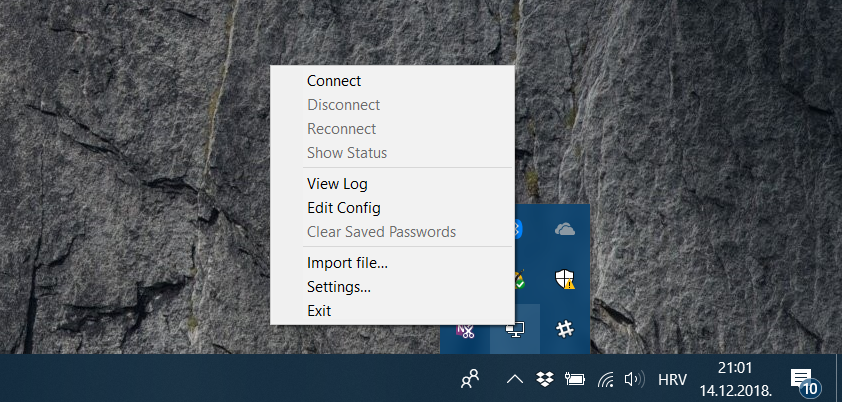
\includegraphics[width=0.7\linewidth]{slike/OpenVPN/win-open-vpn-2}
	\caption[Uvoz klijentske konfiguracije na Windowsima]{Uvoz klijentske konfiguracije na Windowsima}
	\label{fig:win-open-vpn-2}
\end{figure}
\bigbreak
\paragraph*{Instalacija na mobilnim uređajima}
\hfill \smallbreak
Instalacija na Android i iOS sustavima je gotovo identična. Ovdje će biti opisano spajanje na Android 8.1 operacijskom sustavu.\\ Skinite aplikaciju OpenVPN i otvorite ju, bit će vam prikazan početni ekran kao na slici \ref{fig:screenshot20181214-195518}. Odaberite opciju spajanja preko OVPN profila. Profil bi već sada trebao biti dostupan ako ste ga skinuli s interneta, a ako niste onda navigirajte do njega. Odaberite profil client1.ovpn kao što je prikazano na slici \ref{fig:screenshot20181214-195554}.



\begin{figure}[h]
	\centering
	\begin{subfigure}{0.49\textwidth}
		\centering
		\includegraphics[width = 0.5\textwidth]{slike/OpenVPN/Screenshot_20181214-195518}
		\caption{Početni ekran OpenVPN aplikacije}
		\label{fig:screenshot20181214-195518}
	\end{subfigure}
	\begin{subfigure}{0.49\textwidth}
		\centering
		\includegraphics[width = 0.5\textwidth]{slike/OpenVPN/Screenshot_20181214-195554}
		\caption{Odabir klijentske konfiguracije}
		\label{fig:screenshot20181214-195554}
	\end{subfigure}
	\begin{subfigure}{0.49\textwidth}
		\centering
		\includegraphics[width = 0.5\textwidth]{slike/OpenVPN/Screenshot_20181214-195602}
		\caption{Uspješno učitavanje profila}
		\label{fig:screenshot20181214-195602}
	\end{subfigure}
	\begin{subfigure}{0.49\textwidth}
		\centering
		\includegraphics[width = 0.5\textwidth]{slike/OpenVPN/Screenshot_20181214-195614}
		\caption{Profil je uspješno dodan}
		\label{fig:screenshot20181214-195614}
	\end{subfigure}
	\caption{OpenVPN aplikacija}
	\label{fig:combined}
\end{figure}
Nakon toga dobit će te poruku o uspješnom učitavanju profila (slika: \ref{fig:screenshot20181214-195602} ). Stisnite na opciju ADD u gornjem desnom kutu. I na kraju se povežite s VPN poslužteljem pritskajući na sivi gumb (slika: \ref{fig:screenshot20181214-195614}). 




	\newpage
	\bibliographystyle{unsrt}
	\bibliography{literatura}
	

	\newpage
	\begin{appendices}
		\section{Dodatak A: Indeks (slika, tablica, ispisa koda)}
			\renewcommand\listfigurename{}
			\listoffigures
		
	%	\newpage
	%	\section{Dodatak B: Dnevnik sastajanja}

	%	\newpage
	%	\section{Dodatak C: Prikaz aktivnosti grupe}

	%	\newpage
	%	\section{Dodatak D: Plan rada / Pregled rada i stanje ostvarenja}
	\end{appendices}
	
\end{document}
